\documentclass[11pt,a4paper,oneside]{article}
% ---------------------------------------------------------------------
% Catálogo de requisitos del proyecto OLA
% Estructura: ISO/IEC/IEEE 29148:2018 (SRS) · Calidad: ISO/IEC 25010:2011
% Compilar con pdflatex (dos pasadas para el índice).
% ---------------------------------------------------------------------
\usepackage[T1]{fontenc}
\usepackage[utf8]{inputenc}
\usepackage{babel}
\babelprovide[import,main]{spanish}
\setlocalecaption{spanish}{table}{Tabla}
\setlocalecaption{spanish}{listtable}{Índice de tablas}
\setlocalecaption{spanish}{listfigure}{Índice de figuras}
\setlocalecaption{spanish}{contents}{Índice}
\usepackage{textcomp}
\usepackage{microtype}
\usepackage{mathpazo}
\usepackage[scaled=0.92]{helvet}
\usepackage[a4paper, left=2.5cm, right=2.5cm, top=2.8cm, bottom=2.6cm, headheight=15pt]{geometry}
\usepackage[table]{xcolor}
\usepackage{graphicx}
\usepackage{array}
\usepackage{xltabular}
\usepackage{multirow}
\usepackage{enumitem}
\usepackage{titlesec}
\usepackage{fancyhdr}
\usepackage{lastpage}
\usepackage[font=small, labelfont={bf,sf}, skip=6pt]{caption}
\usepackage{tocloft}
\usepackage{float}
\usepackage{needspace}
\usepackage{tikz}
\usetikzlibrary{arrows.meta, positioning, fit, backgrounds}
\usepackage[hidelinks, bookmarksnumbered]{hyperref}

\DeclareUnicodeCharacter{2265}{\ensuremath{\geq}}
\DeclareUnicodeCharacter{2264}{\ensuremath{\leq}}
\DeclareUnicodeCharacter{2212}{\ensuremath{-}}
\DeclareUnicodeCharacter{0394}{\ensuremath{\Delta}}
\DeclareUnicodeCharacter{2192}{\ensuremath{\rightarrow}}
\DeclareUnicodeCharacter{25CF}{\ensuremath{\bullet}}

% ---------- Colores ----------
\definecolor{abisal}{HTML}{0F3849}
\definecolor{marea}{HTML}{1F6F80}
\definecolor{claro}{HTML}{E3EEF0}
\definecolor{zebra}{HTML}{F4F8F8}
\definecolor{borde}{HTML}{B9CBCC}
\definecolor{tenue}{HTML}{465B62}
\arrayrulecolor{borde}

% ---------- Títulos ----------
\titleformat{\section}{\sffamily\LARGE\bfseries\color{abisal}}{\thesection.}{0.6em}{}[\vspace{2pt}{\color{marea}\titlerule[1.2pt]}]
\titleformat{\subsection}{\sffamily\Large\bfseries\color{marea}}{\thesubsection}{0.7em}{}
\titleformat{\subsubsection}{\sffamily\large\bfseries\color{abisal}}{\thesubsubsection}{0.7em}{}
\titlespacing*{\section}{0pt}{0pt}{16pt}
\titlespacing*{\subsection}{0pt}{18pt}{8pt}
\titlespacing*{\subsubsection}{0pt}{14pt}{6pt}
\setcounter{secnumdepth}{3}
\setcounter{tocdepth}{3}

% ---------- Índice ----------
\renewcommand{\cftsecfont}{\sffamily\bfseries}
\renewcommand{\cftsecpagefont}{\sffamily\bfseries}
\renewcommand{\cftsecleader}{\cftdotfill{\cftdotsep}}
\setlength{\cftbeforesecskip}{4pt}
\renewcommand{\cfttoctitlefont}{\sffamily\LARGE\bfseries\color{abisal}}
\renewcommand{\cftlottitlefont}{\sffamily\LARGE\bfseries\color{abisal}}
\renewcommand{\cftloftitlefont}{\sffamily\LARGE\bfseries\color{abisal}}
\setlength{\cftsubsubsecnumwidth}{3.2em}

% ---------- Encabezado y pie ----------
\pagestyle{fancy}
\fancyhf{}
\fancyhead[L]{\sffamily\footnotesize\color{tenue} OLA — Observatorio Litoral de Anomalías térmicas}
\fancyhead[R]{\sffamily\footnotesize\color{tenue} Catálogo de requisitos · v1.0.0}
\newcommand{\pie}{Página \thepage\ de \pageref*{LastPage}}
\fancyfoot[C]{\sffamily\footnotesize\color{tenue} \pie}
\renewcommand{\headrulewidth}{0.4pt}
\renewcommand{\headrule}{{\color{borde}\hrule width\headwidth height\headrulewidth}}
\fancypagestyle{plain}{\fancyhf{}\fancyfoot[C]{\sffamily\footnotesize\color{tenue} \pie}\renewcommand{\headrulewidth}{0pt}}

\renewcommand{\arraystretch}{1.35}
\setlength{\parindent}{0pt}
\setlength{\emergencystretch}{3em}
\raggedbottom
\setlength{\parskip}{6pt}
\setlist[itemize]{topsep=2pt}
\newcolumntype{Y}{>{\raggedright\arraybackslash}X}
\newcommand{\nota}[1]{\begin{center}\colorbox{claro}{\parbox{0.96\textwidth}{\small\sffamily #1}}\end{center}}

\begin{document}
\begin{titlepage}
\centering
{\sffamily\Large\bfseries\color{abisal} UNIVERSIDAD LA SALLE\par}
\vspace{0.6cm}

\includegraphics[width=2.9cm]{figuras/logo_lasalle.png}\par
\vspace{0.8cm}
{\sffamily\large Facultad de Ingenierías y Arquitectura\par}
{\sffamily\large Escuela Profesional de Ingeniería de Software\par}
\vspace{0.4cm}
{\sffamily Docente: Maribel Molina Barriga\par}
\vspace{1.0cm}
{\color{marea}\rule{0.7\textwidth}{1.2pt}\par}
\vspace{0.5cm}
{\sffamily\Huge\bfseries\color{abisal} CATÁLOGO DE REQUISITOS\\[4pt] DEL PROYECTO\par}
\vspace{0.5cm}
{\sffamily\LARGE\color{marea} OLA — Observatorio Litoral de\\ Anomalías térmicas\par}
\vspace{0.5cm}
{\color{marea}\rule{0.7\textwidth}{1.2pt}\par}
\vspace{0.4cm}
{\itshape\color{tenue} Especificación de requisitos de software conforme a ISO/IEC/IEEE 29148:2018,\\ con requisitos de calidad según el modelo ISO/IEC 25010:2011\par}
\vfill
{\sffamily\bfseries Integrantes\par}
\vspace{0.2cm}
{\sffamily Frederick Mares Graos\\ Jhordan Huamani Huamani\\ Jorge Ortiz Castañeda\\ Miguel Angel Flores Leon\\ Piero Adrian Delgado Chipana\par}
\vspace{0.8cm}
{\sffamily Arequipa, 2026\par}
\end{titlepage}


\pagenumbering{roman}\renewcommand{\pie}{\thepage}

\section*{Control del documento}\addcontentsline{toc}{section}{Control del documento}

\Needspace{24\baselineskip}
{\small
\begin{xltabular}{\textwidth}{@{}>{\sffamily\bfseries\raggedright\arraybackslash}p{4.2cm}Y@{}}
\rowcolor{abisal}\textcolor{white}{\sffamily\bfseries\footnotesize Campo} & \textcolor{white}{\sffamily\bfseries\footnotesize Detalle}\\
\endfirsthead
\rowcolor{abisal}\multicolumn{2}{@{}l@{}}{\textcolor{white}{\sffamily\footnotesize (continuación)}}\\
\rowcolor{abisal}\textcolor{white}{\sffamily\bfseries\footnotesize Campo} & \textcolor{white}{\sffamily\bfseries\footnotesize Detalle}\\
\endhead
Proyecto & OLA — Observatorio Litoral de Anomalías térmicas\\ \hline
\rowcolor{zebra}Documento & Catálogo de requisitos del proyecto (Especificación de Requisitos de Software)\\ \hline
Norma de referencia & ISO/IEC/IEEE 29148:2018; modelo de calidad ISO/IEC 25010:2011\\ \hline
\rowcolor{zebra}Versión & 1.0.0\\ \hline
Estado & Para revisión\\ \hline
\rowcolor{zebra}Periodo académico & 2026-II\\ \hline
Repositorio & github.com/Miguel777-rgb/Proyecto\_Calidad\_de\_Software\\ \hline
\end{xltabular}}
\vspace{0.6em}

\subsection*{Historial de versiones}

\Needspace{8\baselineskip}
{\small
\begin{xltabular}{\textwidth}{@{}>{\raggedright\arraybackslash}p{1.4cm}>{\raggedright\arraybackslash}p{2cm}Y>{\raggedright\arraybackslash}p{3.2cm}@{}}
\rowcolor{abisal}\textcolor{white}{\sffamily\bfseries\footnotesize Versión} & \textcolor{white}{\sffamily\bfseries\footnotesize Fecha} & \textcolor{white}{\sffamily\bfseries\footnotesize Descripción} & \textcolor{white}{\sffamily\bfseries\footnotesize Responsable}\\
\endfirsthead
\rowcolor{abisal}\multicolumn{4}{@{}l@{}}{\textcolor{white}{\sffamily\footnotesize (continuación)}}\\
\rowcolor{abisal}\textcolor{white}{\sffamily\bfseries\footnotesize Versión} & \textcolor{white}{\sffamily\bfseries\footnotesize Fecha} & \textcolor{white}{\sffamily\bfseries\footnotesize Descripción} & \textcolor{white}{\sffamily\bfseries\footnotesize Responsable}\\
\endhead
1.0.0 & 24/09/2026 & Versión inicial del catálogo de requisitos, estructurada según ISO/IEC/IEEE 29148:2018, con requisitos no funcionales agrupados por las características de ISO/IEC 25010:2011 y criterios de aceptación para cada requisito funcional. Parte de la línea base de requisitos v1.6 (Apéndice C). & Equipo del proyecto OLA\\ \hline
\end{xltabular}}
\vspace{0.6em}

\subsection*{Aprobaciones}

\Needspace{14\baselineskip}
{\small
\begin{xltabular}{\textwidth}{@{}>{\raggedright\arraybackslash}p{3.2cm}Y>{\raggedright\arraybackslash}p{3.6cm}>{\raggedright\arraybackslash}p{2.4cm}@{}}
\rowcolor{abisal}\textcolor{white}{\sffamily\bfseries\footnotesize Rol} & \textcolor{white}{\sffamily\bfseries\footnotesize Nombre} & \textcolor{white}{\sffamily\bfseries\footnotesize Firma} & \textcolor{white}{\sffamily\bfseries\footnotesize Fecha}\\
\endfirsthead
\rowcolor{abisal}\multicolumn{4}{@{}l@{}}{\textcolor{white}{\sffamily\footnotesize (continuación)}}\\
\rowcolor{abisal}\textcolor{white}{\sffamily\bfseries\footnotesize Rol} & \textcolor{white}{\sffamily\bfseries\footnotesize Nombre} & \textcolor{white}{\sffamily\bfseries\footnotesize Firma} & \textcolor{white}{\sffamily\bfseries\footnotesize Fecha}\\
\endhead
Product Owner & Miguel Angel Flores Leon &  & \\ \hline
Scrum Master & Jorge Ortiz Castañeda &  & \\ \hline
Revisora & Maribel Molina Barriga &  & \\ \hline
\end{xltabular}}
\vspace{0.6em}

\clearpage\tableofcontents\clearpage\listoftables\vspace{1cm}\listoffigures\clearpage\pagenumbering{arabic}\renewcommand{\pie}{Página \thepage\ de \pageref*{LastPage}}

\section{Introducción}

\Needspace{26\baselineskip}\subsection{Propósito}

Este documento especifica los requisitos de software del sistema OLA siguiendo la estructura de la Especificación de Requisitos de Software (SRS) de la norma ISO/IEC/IEEE 29148:2018. Reúne en un catálogo único los requisitos funcionales, los requisitos no funcionales (organizados según las características de calidad de ISO/IEC 25010:2011), los requisitos de interfaz, los requisitos lógicos de datos y las restricciones de diseño, junto con los criterios de aceptación y el método con que se verifica cada uno.



Está dirigido a la docente del curso, como evaluadora, y al equipo de desarrollo, como referencia para comprobar que cada funcionalidad construida responde a un requisito documentado y verificable.



\Needspace{26\baselineskip}\subsection{Alcance}

\textbf{OLA} (Observatorio Litoral de Anomalías térmicas) es una aplicación web que toma el dataset abierto de Anomalía de la Temperatura Superficial del Mar (ATSM) publicado por IMARPE/PRODUCE, clasifica el estado térmico de los 10 laboratorios costeros del litoral peruano en \textbf{cálido}, \textbf{neutro} o \textbf{frío}, lo muestra en un mapa interactivo, grafica y compara su histórico, estima la tendencia de los próximos días y avisa a los usuarios suscritos cuando una zona mantiene una anomalía sostenida.



Los objetivos del sistema, a los que se vincula cada requisito funcional (sección 4.4), son:



\Needspace{20\baselineskip}
{\small
\begin{xltabular}{\textwidth}{@{}>{\sffamily\bfseries}p{1.5cm}Y>{\raggedright\arraybackslash}p{3cm}@{}}
\caption{Objetivos del sistema}\label{tab:obj}\\
\rowcolor{abisal}\textcolor{white}{\sffamily\bfseries\footnotesize ID} & \textcolor{white}{\sffamily\bfseries\footnotesize Objetivo} & \textcolor{white}{\sffamily\bfseries\footnotesize Requisitos}\\
\endfirsthead
\rowcolor{abisal}\multicolumn{3}{@{}l@{}}{\textcolor{white}{\sffamily\footnotesize Objetivos del sistema (continuación)}}\\
\rowcolor{abisal}\textcolor{white}{\sffamily\bfseries\footnotesize ID} & \textcolor{white}{\sffamily\bfseries\footnotesize Objetivo} & \textcolor{white}{\sffamily\bfseries\footnotesize Requisitos}\\
\endhead
OBJ-01 & Informar el estado térmico actual de la costa, en un vistazo y desde el celular, indicando de cuándo es el dato. & RF-04\\ \hline
\rowcolor{zebra}OBJ-02 & Detectar las anomalías sostenidas y comunicarlas a las personas que siguen cada zona. & RF-01, RF-03, RF-07\\ \hline
OBJ-03 & Facilitar el análisis histórico de una zona desde 1970 y su comparación con otras. & RF-05, RF-06\\ \hline
\rowcolor{zebra}OBJ-04 & Ofrecer una estimación aproximada, claramente marcada como tal, de la clasificación de los próximos días. & RF-02\\ \hline
OBJ-05 & Mantener el dataset oficial actualizado y gestionar las cuentas y zonas de interés de los usuarios. & RF-07, RF-08\\ \hline
\end{xltabular}}
\vspace{0.6em}

\textbf{Fuera de alcance en esta versión:}



\begin{itemize}[leftmargin=1.4em, itemsep=2pt]
\item Predecir eventos El Niño o La Niña con certeza científica; esa función corresponde oficialmente al ENFEN.
\item Reemplazar los boletines técnicos de IMARPE; OLA los complementa.
\item Aplicación móvil nativa; OLA es una aplicación web responsiva.
\item Envío de SMS; los avisos llegan por correo electrónico y dentro de la aplicación.
\item Importación programada del dataset; la carga es manual y la realiza el administrador.
\item Pagos o cualquier modelo de monetización.
\end{itemize}


\Needspace{26\baselineskip}\subsection{Visión general del producto}

\Needspace{14\baselineskip}\subsubsection{Perspectiva del producto}

\textbf{Contexto.} El litoral peruano, bajo la influencia de la corriente de Humboldt, es muy sensible a las variaciones de la temperatura del mar. Un calentamiento o enfriamiento sostenido altera la disponibilidad de los recursos pesqueros y la economía de miles de pescadores artesanales. IMARPE mide a diario la temperatura en sus laboratorios costeros y publica la anomalía como dato abierto: el archivo cubre de 1970 a 2026 con 125,701 registros de tres columnas (fecha de medición, laboratorio costero y anomalía en °C).



\textbf{Problemática.} El dato es público, pero no llega a quien más lo necesita. Se publica como un CSV de más de cien mil filas, útil para especialistas pero no para un pescador que consulta desde el celular; un valor aislado no indica si la situación es normal ni si se sostiene en el tiempo; no existe un mecanismo que avise a quien sigue una zona; y el dato llega con retraso y con huecos (el laboratorio de Matarani dejó de medir en 2016) que un lector no especialista no puede advertir.



\textbf{Relación con otros sistemas.} OLA es un sistema nuevo e independiente. No se integra formalmente con los sistemas de IMARPE ni del ENFEN: consume el archivo público que el administrador carga en la aplicación y opera como una capa de visualización y alerta. La Figura \ref{fig:arq} muestra sus componentes y los sistemas externos con los que se comunica.



\begin{figure}[H]
\centering
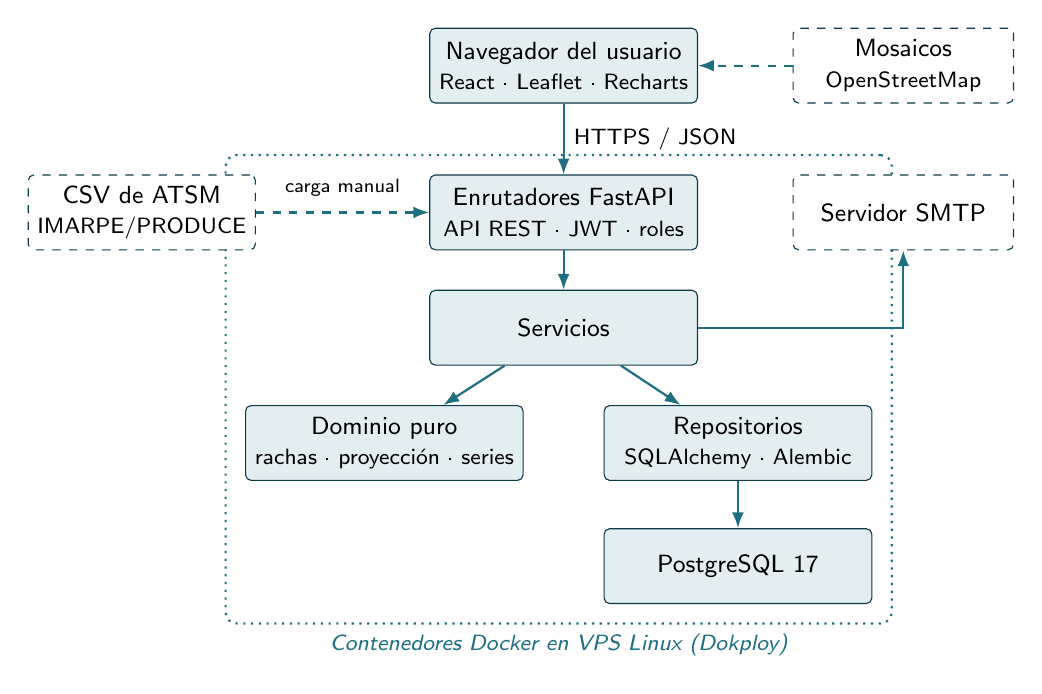
\begin{tikzpicture}[font=\sffamily\small,
  caja/.style={draw=abisal, fill=claro, rounded corners=2pt, minimum width=3.4cm, minimum height=0.95cm, align=center},
  ext/.style={draw=abisal, dashed, fill=white, rounded corners=2pt, minimum width=2.8cm, minimum height=0.95cm, align=center},
  flecha/.style={-{Latex[length=2mm]}, draw=marea, thick}]
\node[caja] (web) {Navegador del usuario\\\footnotesize React · Leaflet · Recharts};
\node[caja, below=0.9cm of web] (api) {Enrutadores FastAPI\\\footnotesize API REST · JWT · roles};
\node[caja, below=0.5cm of api] (serv) {Servicios};
\node[caja, below left=0.5cm and -1.2cm of serv] (dom) {Dominio puro\\\footnotesize rachas · proyección · series};
\node[caja, below right=0.5cm and -1.2cm of serv] (repo) {Repositorios\\\footnotesize SQLAlchemy · Alembic};
\node[caja, below=0.6cm of repo] (db) {PostgreSQL 17};
\node[ext, right=1.2cm of api] (smtp) {Servidor SMTP};
\node[ext, left=2.2cm of api] (csv) {CSV de ATSM\\\footnotesize IMARPE/PRODUCE};
\node[ext, right=1.2cm of web] (osm) {Mosaicos\\\footnotesize OpenStreetMap};
\begin{scope}[on background layer]
\node[draw=marea, dotted, thick, rounded corners, fit=(api)(serv)(dom)(repo)(db), inner sep=7pt, label={[font=\sffamily\footnotesize\itshape, text=marea]below:Contenedores Docker en VPS Linux (Dokploy)}] {};
\end{scope}
\draw[flecha] (web) -- node[right, font=\sffamily\footnotesize]{HTTPS / JSON} (api);
\draw[flecha] (api) -- (serv);
\draw[flecha] (serv) -- (dom);
\draw[flecha] (serv) -- (repo);
\draw[flecha] (repo) -- (db);
\draw[flecha] (serv.east) -| (smtp.south);
\draw[flecha, dashed] (csv) -- node[above=2pt, font=\sffamily\scriptsize]{carga manual} (api);
\draw[flecha, dashed] (osm) -- (web);
\end{tikzpicture}
\caption{Perspectiva del producto: componentes de OLA y sistemas externos.}
\label{fig:arq}
\end{figure}


\Needspace{14\baselineskip}\subsubsection{Funciones del producto}

De forma resumida, el sistema:



\begin{itemize}[leftmargin=1.4em, itemsep=2pt]
\item Clasifica automáticamente el estado térmico de cada zona costera y detecta anomalías sostenidas (RF-01).
\item Estima la tendencia térmica de los próximos 3 a 7 días (RF-02).
\item Notifica a los usuarios suscritos el inicio y el fin de cada episodio de alerta (RF-03).
\item Muestra el estado de las 10 zonas en un mapa interactivo (RF-04).
\item Grafica el histórico de una zona y compara varias zonas en un mismo periodo (RF-05, RF-06).
\item Permite el registro, la autenticación y la suscripción a zonas de interés (RF-07).
\item Permite al administrador importar y actualizar el dataset de IMARPE (RF-08).
\end{itemize}


La Figura \ref{fig:cu} muestra estas funciones como casos de uso agrupados por actor, y la Tabla \ref{tab:uc} las relaciona con los requisitos funcionales.



\begin{figure}[H]
\centering
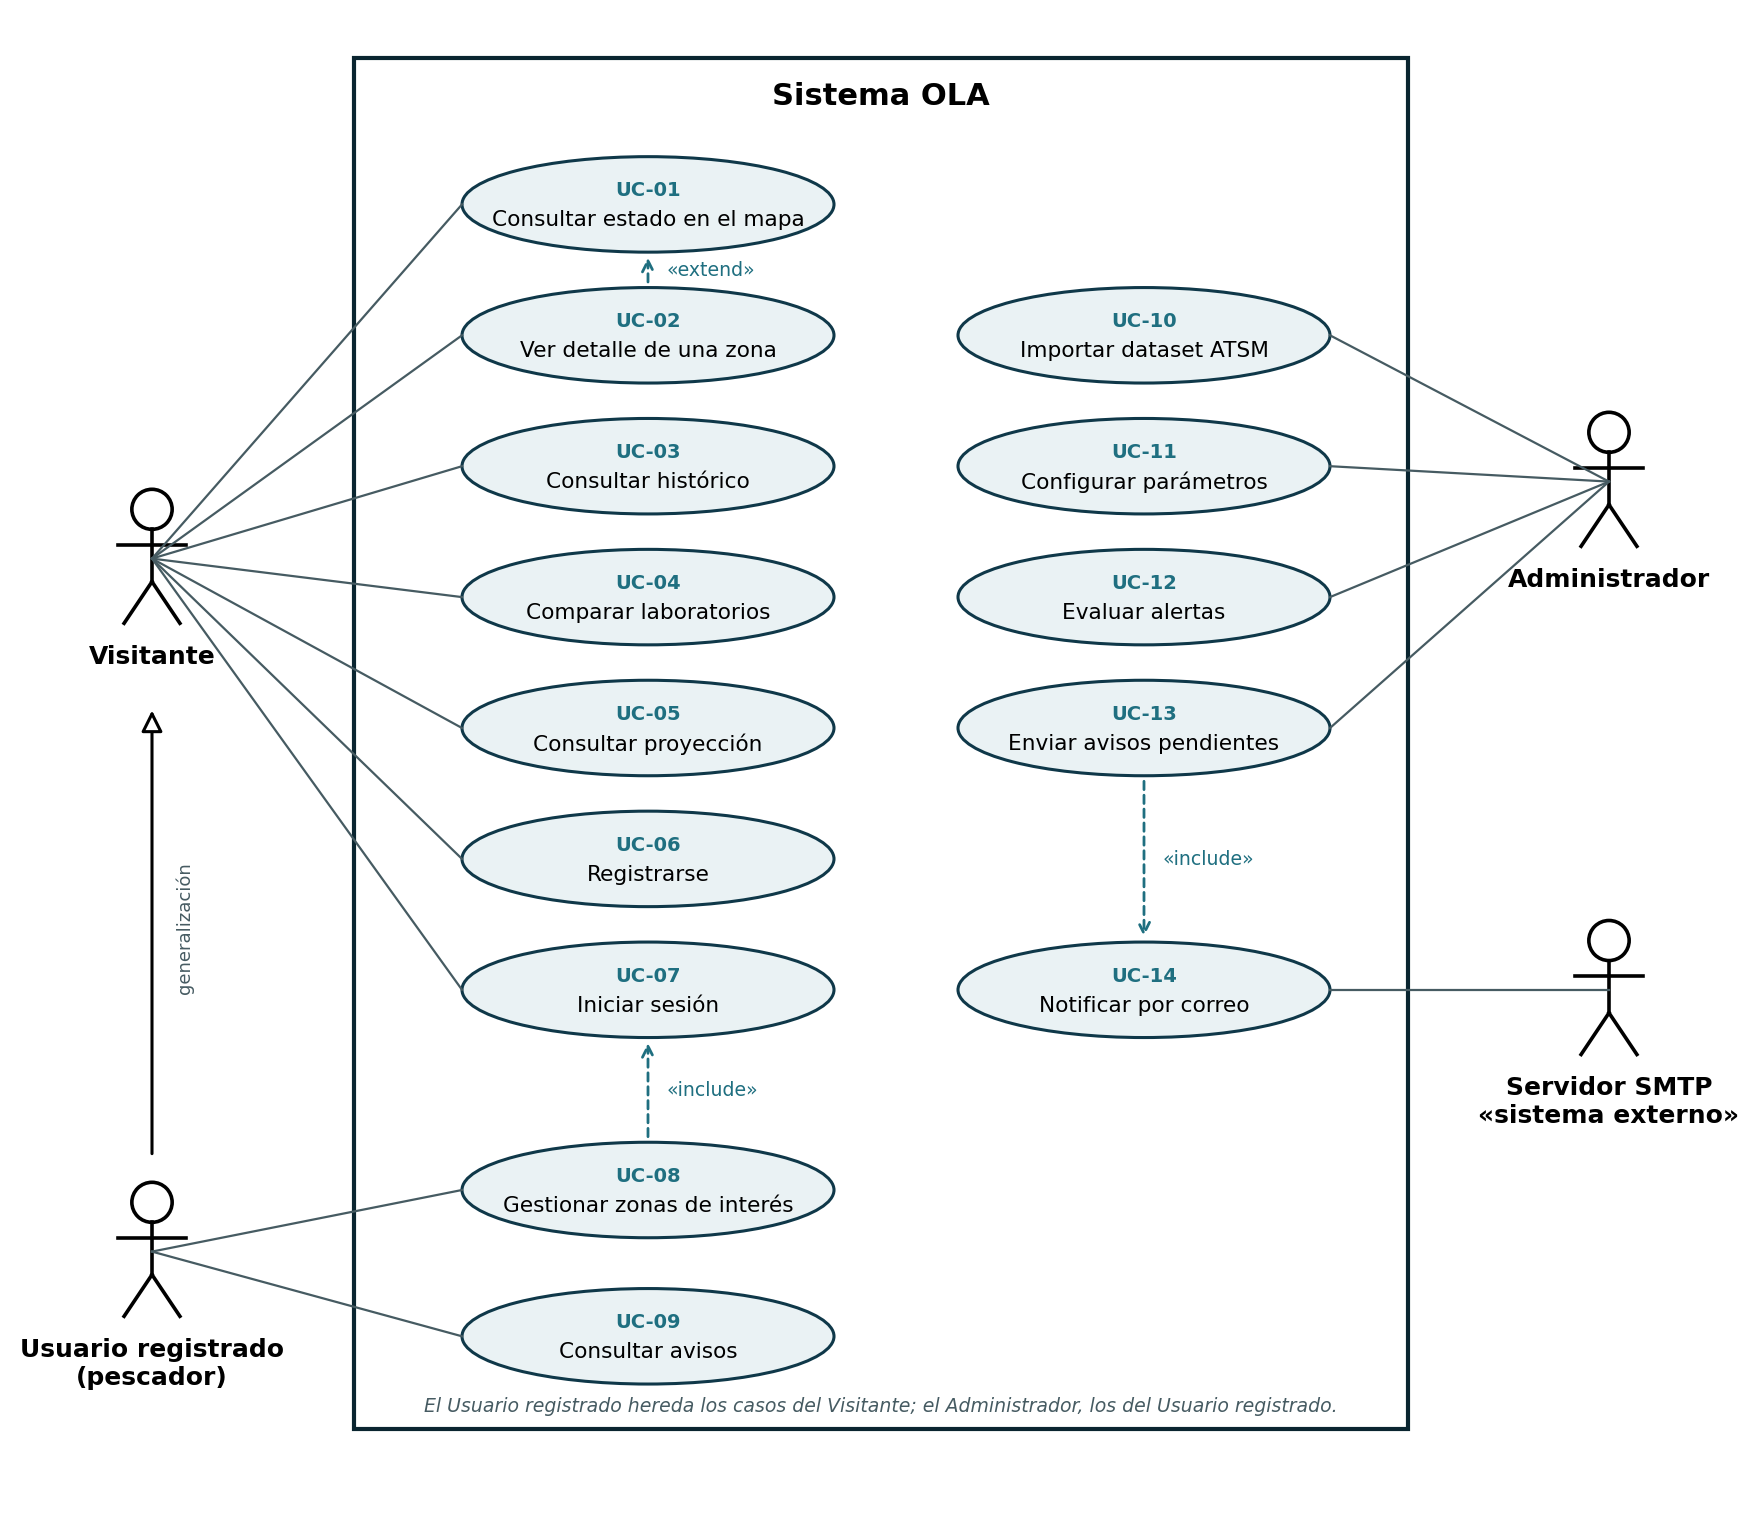
\includegraphics[width=0.86\textwidth]{figuras/casos_uso.png}
\caption{Diagrama de casos de uso del sistema OLA.}
\label{fig:cu}
\end{figure}


\Needspace{12\baselineskip}
{\small
\begin{xltabular}{\textwidth}{@{}>{\sffamily\bfseries}p{1.5cm}Y>{\raggedright\arraybackslash}p{3.6cm}>{\raggedright\arraybackslash}p{2.6cm}@{}}
\caption{Casos de uso y requisitos funcionales que los cubren}\label{tab:uc}\\
\rowcolor{abisal}\textcolor{white}{\sffamily\bfseries\footnotesize ID} & \textcolor{white}{\sffamily\bfseries\footnotesize Caso de uso} & \textcolor{white}{\sffamily\bfseries\footnotesize Actor principal} & \textcolor{white}{\sffamily\bfseries\footnotesize RF}\\
\endfirsthead
\rowcolor{abisal}\multicolumn{4}{@{}l@{}}{\textcolor{white}{\sffamily\footnotesize Casos de uso y requisitos funcionales que los cubren (continuación)}}\\
\rowcolor{abisal}\textcolor{white}{\sffamily\bfseries\footnotesize ID} & \textcolor{white}{\sffamily\bfseries\footnotesize Caso de uso} & \textcolor{white}{\sffamily\bfseries\footnotesize Actor principal} & \textcolor{white}{\sffamily\bfseries\footnotesize RF}\\
\endhead
UC-01 & Consultar el estado en el mapa & Visitante & RF-04\\ \hline
\rowcolor{zebra}UC-02 & Ver el detalle de una zona & Visitante & RF-04\\ \hline
UC-03 & Consultar el histórico & Visitante & RF-05\\ \hline
\rowcolor{zebra}UC-04 & Comparar laboratorios & Visitante & RF-06\\ \hline
UC-05 & Consultar la proyección & Visitante & RF-02\\ \hline
\rowcolor{zebra}UC-06 & Registrarse & Visitante & RF-07\\ \hline
UC-07 & Iniciar sesión & Visitante & RF-07\\ \hline
\rowcolor{zebra}UC-08 & Gestionar zonas de interés & Usuario registrado & RF-07, RF-03\\ \hline
UC-09 & Consultar avisos & Usuario registrado & RF-03\\ \hline
\rowcolor{zebra}UC-10 & Importar el dataset ATSM & Administrador & RF-08\\ \hline
UC-11 & Configurar parámetros & Administrador & RF-01, RF-04\\ \hline
\rowcolor{zebra}UC-12 & Evaluar alertas & Administrador & RF-01, RF-03\\ \hline
UC-13 & Enviar avisos pendientes & Administrador & RF-03\\ \hline
\rowcolor{zebra}UC-14 & Notificar por correo & Servidor SMTP & RF-03\\ \hline
\end{xltabular}}
\vspace{0.6em}

\Needspace{14\baselineskip}\subsubsection{Características de los usuarios}

\Needspace{14\baselineskip}
{\small
\begin{xltabular}{\textwidth}{@{}>{\sffamily\bfseries\raggedright\arraybackslash}p{3.2cm}YY@{}}
\caption{Características de los usuarios}\label{tab:usuarios}\\
\rowcolor{abisal}\textcolor{white}{\sffamily\bfseries\footnotesize Usuario} & \textcolor{white}{\sffamily\bfseries\footnotesize Perfil} & \textcolor{white}{\sffamily\bfseries\footnotesize Necesidad principal}\\
\endfirsthead
\rowcolor{abisal}\multicolumn{3}{@{}l@{}}{\textcolor{white}{\sffamily\footnotesize Características de los usuarios (continuación)}}\\
\rowcolor{abisal}\textcolor{white}{\sffamily\bfseries\footnotesize Usuario} & \textcolor{white}{\sffamily\bfseries\footnotesize Perfil} & \textcolor{white}{\sffamily\bfseries\footnotesize Necesidad principal}\\
\endhead
Visitante & Cualquier persona que usa la aplicación sin iniciar sesión. & Consultar el estado, el histórico, la comparación y la proyección de las zonas.\\ \hline
\rowcolor{zebra}Usuario registrado (pescador artesanal) & Usuario final, con alfabetización digital posiblemente limitada; accede sobre todo desde el celular, a veces al sol. & Saber, sin interpretar datos técnicos, si el mar de su zona está más cálido o frío de lo normal, y recibir avisos a tiempo.\\ \hline
Administrador & Miembro del equipo del proyecto, con conocimientos técnicos. & Importar el dataset, ajustar los parámetros de detección y supervisar la evaluación de alertas y el envío de avisos.\\ \hline
\end{xltabular}}
\vspace{0.6em}

Además de los usuarios, intervienen dos actores externos: el \textbf{servidor SMTP}, que entrega los avisos por correo, e \textbf{IMARPE/PRODUCE}, fuente del archivo CSV. Los interesados en el sistema son los pescadores artesanales, el administrador, IMARPE/PRODUCE (que su dato se use con atribución y sin tergiversar su alcance) y la docente del curso, como evaluadora del proceso de calidad.



\Needspace{14\baselineskip}\subsubsection{Limitaciones}

\begin{itemize}[leftmargin=1.4em, itemsep=2pt]
\item \textbf{Dependencia de los datos:} el sistema depende de la disponibilidad y del formato del dataset público de IMARPE; un cambio en sus columnas exigiría ajustar el importador (RF-08).
\item \textbf{Carácter no oficial:} las clasificaciones y proyecciones son orientativas; el sistema no sustituye los comunicados oficiales del ENFEN ni los boletines de IMARPE.
\item \textbf{Licencia de datos:} el uso del dataset debe respetar la licencia de datos abiertos del Estado peruano, que exige atribución.
\item \textbf{Tiempo y equipo:} el proyecto se desarrolla dentro del cronograma del curso (Hito 1: 12–17/10/2026; Hito 2: primera semana de diciembre de 2026) con un equipo de cinco integrantes.
\item \textbf{Infraestructura:} el sistema se despliega en un VPS propio del equipo, sin acuerdo de nivel de servicio productivo.
\end{itemize}


\Needspace{26\baselineskip}\subsection{Definiciones, acrónimos y abreviaturas}

\Needspace{12\baselineskip}
{\small
\begin{xltabular}{\textwidth}{@{}>{\sffamily\bfseries\raggedright\arraybackslash}p{4.2cm}Y@{}}
\caption{Definiciones, acrónimos y abreviaturas}\label{tab:defs}\\
\rowcolor{abisal}\textcolor{white}{\sffamily\bfseries\footnotesize Término} & \textcolor{white}{\sffamily\bfseries\footnotesize Definición}\\
\endfirsthead
\rowcolor{abisal}\multicolumn{2}{@{}l@{}}{\textcolor{white}{\sffamily\footnotesize Definiciones, acrónimos y abreviaturas (continuación)}}\\
\rowcolor{abisal}\textcolor{white}{\sffamily\bfseries\footnotesize Término} & \textcolor{white}{\sffamily\bfseries\footnotesize Definición}\\
\endhead
ATSM & Anomalía de la Temperatura Superficial del Mar: diferencia, en °C, entre la temperatura medida y su valor normal para esa fecha y lugar.\\ \hline
\rowcolor{zebra}Laboratorio costero (zona) & Estación de IMARPE que mide la temperatura del mar. OLA trabaja con 10: Tumbes, Paita, San José, Chicama, Chimbote, Huacho, Callao, Pisco, Matarani e Ilo.\\ \hline
Racha & Sucesión de mediciones consecutivas de una zona fuera del rango neutro y con el mismo signo.\\ \hline
\rowcolor{zebra}Episodio de alerta & Racha que alcanza la longitud mínima configurada (5 registros por defecto), con fecha de inicio, fecha de fin y estado cálido o frío.\\ \hline
Fecha de referencia & Fecha de la medición más reciente cargada en el sistema; sirve de «hoy» para todos los cálculos.\\ \hline
\rowcolor{zebra}Aviso & Notificación dirigida a un usuario sobre el inicio o el fin de un episodio, entregada por correo y dentro de la aplicación.\\ \hline
Criterio de aceptación & Condición verificable que el sistema debe cumplir para que un requisito se considere satisfecho.\\ \hline
\rowcolor{zebra}IMARPE / PRODUCE & Instituto del Mar del Perú / Ministerio de la Producción.\\ \hline
ENFEN & Comisión Multisectorial encargada del Estudio Nacional del Fenómeno El Niño.\\ \hline
\rowcolor{zebra}RF / RNF / RN / IRQ / RD & Requisito funcional / requisito no funcional / regla de negocio / requisito de información / restricción de diseño.\\ \hline
SRS & Software Requirements Specification (Especificación de Requisitos de Software).\\ \hline
\rowcolor{zebra}API REST & Interfaz de programación basada en HTTP que usa el frontend para comunicarse con el backend.\\ \hline
JWT & JSON Web Token: credencial firmada que identifica la sesión del usuario.\\ \hline
\rowcolor{zebra}WCAG & Web Content Accessibility Guidelines, pautas de accesibilidad del W3C.\\ \hline
SMTP & Simple Mail Transfer Protocol, protocolo de envío de correo.\\ \hline
\rowcolor{zebra}VPS & Virtual Private Server (servidor privado virtual).\\ \hline
\end{xltabular}}
\vspace{0.6em}

\section{Referencias}

\begin{enumerate}[label={[\arabic*]}, leftmargin=2.2em, itemsep=3pt]
\item ISO/IEC/IEEE 29148:2018, \emph{Systems and software engineering — Life cycle processes — Requirements engineering}.
\item ISO/IEC 25010:2011, \emph{Systems and software engineering — Systems and software Quality Requirements and Evaluation (SQuaRE) — System and software quality models}.
\item W3C, \emph{Web Content Accessibility Guidelines (WCAG) 2.2}, W3C Recommendation, 2023.
\item IMARPE/PRODUCE, \emph{Anomalía de la Temperatura Superficial del Mar (ATSM) de los laboratorios costeros del IMARPE}, Plataforma Nacional de Datos Abiertos, \url{https://www.datosabiertos.gob.pe}.
\item Comisión Multisectorial ENFEN, \emph{Definición operacional de los eventos El Niño costero y La Niña costera en el Perú}, Nota Técnica ENFEN 01-2024.
\item Equipo OLA, \emph{Matriz de trazabilidad} (\texttt{docs/trazabilidad.md}) y \emph{Registro de decisiones de diseño} (\texttt{docs/decisiones.md}), repositorio del proyecto.
\end{enumerate}


\clearpage\section{Requisitos específicos}

Esta sección contiene los requisitos del sistema. Cada requisito se redacta con la forma «El sistema deberá…», tiene un identificador único y los atributos que recomienda ISO/IEC/IEEE 29148:2018 para su gestión. La Tabla \ref{tab:attr} describe esos atributos.



\Needspace{12\baselineskip}
{\small
\begin{xltabular}{\textwidth}{@{}>{\sffamily\bfseries\raggedright\arraybackslash}p{4cm}Y@{}}
\caption{Atributos de los requisitos}\label{tab:attr}\\
\rowcolor{abisal}\textcolor{white}{\sffamily\bfseries\footnotesize Atributo} & \textcolor{white}{\sffamily\bfseries\footnotesize Descripción y valores}\\
\endfirsthead
\rowcolor{abisal}\multicolumn{2}{@{}l@{}}{\textcolor{white}{\sffamily\footnotesize Atributos de los requisitos (continuación)}}\\
\rowcolor{abisal}\textcolor{white}{\sffamily\bfseries\footnotesize Atributo} & \textcolor{white}{\sffamily\bfseries\footnotesize Descripción y valores}\\
\endhead
Identificador & Código único e invariable: RF-nn (funcional), RNF-nn (no funcional), RN-nn (regla de negocio), IRQ-nn (información), RD-nn (restricción de diseño).\\ \hline
\rowcolor{zebra}Enunciado & Descripción del requisito en forma «El sistema deberá…», necesaria, no ambigua, completa, singular, factible y verificable.\\ \hline
Requisitos derivados & Descomposición del requisito en requisitos más específicos (RF-nn.m).\\ \hline
\rowcolor{zebra}Justificación & Razón por la que el requisito existe o tiene su forma actual.\\ \hline
Fuente & Origen del requisito: interesado, documento o análisis que lo motiva.\\ \hline
\rowcolor{zebra}Prioridad & Alta, Media o Baja, según su aporte a los objetivos del sistema.\\ \hline
Dificultad & Alta, Media o Baja, según el esfuerzo técnico estimado.\\ \hline
\rowcolor{zebra}Riesgo & Alto, Medio o Bajo, según la probabilidad de que el requisito no se cumpla o cambie.\\ \hline
Estabilidad & Alta, Media o Baja, según la probabilidad de que el requisito cambie.\\ \hline
\rowcolor{zebra}Dependencias & Otros requisitos, reglas o datos de los que depende.\\ \hline
Método de verificación & Inspección (I), Análisis (A), Demostración (D) o Prueba (P), según la sección 4.1.\\ \hline
\rowcolor{zebra}Criterios de aceptación & Condiciones verificables (CA-nn.m) en forma «Dado… cuando… entonces…».\\ \hline
Estado & Propuesto, Aprobado, Implementado o Verificado.\\ \hline
\end{xltabular}}
\vspace{0.6em}

\Needspace{26\baselineskip}\subsection{Requisitos funcionales}

\Needspace{14\baselineskip}\subsubsection{Resumen}

\Needspace{24\baselineskip}
{\small
\begin{xltabular}{\textwidth}{@{}>{\sffamily\bfseries}p{1.5cm}Y>{\raggedright\arraybackslash}p{1.9cm}>{\raggedright\arraybackslash}p{1.9cm}>{\raggedright\arraybackslash}p{2.1cm}@{}}
\caption{Resumen de requisitos funcionales}\label{tab:rfres}\\
\rowcolor{abisal}\textcolor{white}{\sffamily\bfseries\footnotesize ID} & \textcolor{white}{\sffamily\bfseries\footnotesize Requisito} & \textcolor{white}{\sffamily\bfseries\footnotesize Prioridad} & \textcolor{white}{\sffamily\bfseries\footnotesize Dificultad} & \textcolor{white}{\sffamily\bfseries\footnotesize Estado}\\
\endfirsthead
\rowcolor{abisal}\multicolumn{5}{@{}l@{}}{\textcolor{white}{\sffamily\footnotesize Resumen de requisitos funcionales (continuación)}}\\
\rowcolor{abisal}\textcolor{white}{\sffamily\bfseries\footnotesize ID} & \textcolor{white}{\sffamily\bfseries\footnotesize Requisito} & \textcolor{white}{\sffamily\bfseries\footnotesize Prioridad} & \textcolor{white}{\sffamily\bfseries\footnotesize Dificultad} & \textcolor{white}{\sffamily\bfseries\footnotesize Estado}\\
\endhead
RF-01 & Detección de anomalía térmica sostenida & Alta & Alta & Verificado\\ \hline
\rowcolor{zebra}RF-02 & Proyección de tendencia a corto plazo & Media & Alta & Verificado\\ \hline
RF-03 & Notificación automática & Media & Alta & Verificado\\ \hline
\rowcolor{zebra}RF-04 & Mapa interactivo de estado por zona & Alta & Media & Verificado\\ \hline
RF-05 & Gráficos históricos por laboratorio & Media & Media & Verificado\\ \hline
\rowcolor{zebra}RF-06 & Comparación entre laboratorios costeros & Baja & Media & Verificado\\ \hline
RF-07 & Registro y autenticación de usuarios & Alta & Baja & Verificado\\ \hline
\rowcolor{zebra}RF-08 & Importación y actualización del dataset ATSM & Alta & Baja & Verificado\\ \hline
\end{xltabular}}
\vspace{0.6em}

\Needspace{14\baselineskip}\subsubsection{Reglas de negocio}

Las reglas de negocio restringen el comportamiento de los requisitos funcionales. Los valores configurables pueden cambiarse desde la aplicación dentro del rango indicado en RN-17.



\Needspace{12\baselineskip}
{\footnotesize
\begin{xltabular}{\textwidth}{@{}>{\sffamily\bfseries}p{1.3cm}Y>{\raggedright\arraybackslash}p{2.6cm}>{\raggedright\arraybackslash}p{2.1cm}@{}}
\caption{Reglas de negocio}\label{tab:rn}\\
\rowcolor{abisal}\textcolor{white}{\sffamily\bfseries\footnotesize ID} & \textcolor{white}{\sffamily\bfseries\footnotesize Regla} & \textcolor{white}{\sffamily\bfseries\footnotesize Valor por defecto} & \textcolor{white}{\sffamily\bfseries\footnotesize RF}\\
\endfirsthead
\rowcolor{abisal}\multicolumn{4}{@{}l@{}}{\textcolor{white}{\sffamily\footnotesize Reglas de negocio (continuación)}}\\
\rowcolor{abisal}\textcolor{white}{\sffamily\bfseries\footnotesize ID} & \textcolor{white}{\sffamily\bfseries\footnotesize Regla} & \textcolor{white}{\sffamily\bfseries\footnotesize Valor por defecto} & \textcolor{white}{\sffamily\bfseries\footnotesize RF}\\
\endhead
RN-01 & Una medición es \textbf{cálida} si su anomalía es mayor que +umbral, \textbf{fría} si es menor que −umbral y \textbf{neutra} en otro caso. El límite es exclusivo: exactamente ±0.5 °C es neutro. & Umbral 0.5 °C (configurable) & RF-01, RF-04\\ \hline
\rowcolor{zebra}RN-02 & Una racha se cuenta por \textbf{registros consecutivos} del mismo signo fuera del rango neutro; un valor neutro o un cambio de signo la interrumpe. & — & RF-01\\ \hline
RN-03 & Entre dos mediciones de una racha se toleran días faltantes; si el hueco supera la tolerancia, la racha se reinicia. & 2 días (configurable) & RF-01\\ \hline
\rowcolor{zebra}RN-04 & Una racha se convierte en episodio de alerta al alcanzar la longitud mínima. & 5 registros (configurable) & RF-01\\ \hline
RN-05 & La \textbf{fecha de referencia} de todos los cálculos es la de la medición más reciente del sistema, nunca el reloj del servidor. & — & RF-01, RF-02, RF-04\\ \hline
\rowcolor{zebra}RN-06 & El estado de cada zona en el mapa se calcula sobre el \textbf{promedio} de sus mediciones en la ventana del mapa, contada hacia atrás desde la fecha de referencia. & 5 días (configurable) & RF-04\\ \hline
RN-07 & Una zona sin mediciones dentro de la vigencia se muestra como «sin datos recientes» y no se clasifica. & 7 días (configurable) & RF-04\\ \hline
\rowcolor{zebra}RN-08 & La proyección usa las últimas mediciones disponibles de la zona y requiere al menos 3 para calcularse. & 30 mediciones & RF-02\\ \hline
RN-09 & El horizonte de proyección está entre 3 y 7 días. & 5 días & RF-02\\ \hline
\rowcolor{zebra}RN-10 & La confianza de la proyección es \textbf{alta} si la cobertura de la ventana es ≥ 70 \%, \textbf{media} si es ≥ 40 \% y \textbf{baja} en otro caso, o si el último dato supera la vigencia. & — & RF-02\\ \hline
RN-11 & Cada episodio genera como máximo un aviso por usuario, canal y momento (inicio o fin), aunque se reevalúe varias veces. & — & RF-03\\ \hline
\rowcolor{zebra}RN-12 & Un usuario que se suscribe a una zona con alerta vigente recibe el aviso de inicio de ese episodio. & — & RF-03\\ \hline
RN-13 & El histórico se agrupa según el rango: diario hasta 1 año, promedio semanal hasta 5 años y mensual por encima. & Rango inicial: 90 días & RF-05, RF-06\\ \hline
\rowcolor{zebra}RN-14 & La comparación admite entre 2 y 4 laboratorios. & — & RF-06\\ \hline
RN-15 & La contraseña debe tener al menos 8 caracteres y no superar 72 bytes; el correo electrónico es único. & — & RF-07\\ \hline
\rowcolor{zebra}RN-16 & Una fila del CSV se rechaza si su fecha no es válida, su laboratorio no está en el catálogo, su anomalía no es numérica o usa coma decimal. El archivo no puede superar 50 MB. & — & RF-08\\ \hline
RN-17 & Rangos admitidos: umbral 0.1–5.0 °C; racha 2–60 registros; huecos 0–30 días; vigencia 1–365 días; ventana del mapa 1–60 días. & — & RF-01, RF-04\\ \hline
\rowcolor{zebra}RN-18 & Reimportar una medición existente actualiza su valor si cambió y no la duplica. & — & RF-08\\ \hline
\end{xltabular}}
\vspace{0.6em}

\Needspace{26\baselineskip}\subsubsection{RF-01 Detección de anomalía térmica sostenida}

\begin{xltabular}{\textwidth}{@{}>{\columncolor{claro}\sffamily\bfseries\small\raggedright\arraybackslash}p{3.6cm}>{\small\raggedright\arraybackslash}X@{}}
\rowcolor{abisal}\textcolor{white}{RF-01} & \textcolor{white}{\sffamily\bfseries Detección de anomalía térmica sostenida}\\
\endfirsthead
\rowcolor{abisal}\textcolor{white}{RF-01} & \textcolor{white}{\sffamily\bfseries Detección de anomalía térmica sostenida \textmd{\small(continuación)}}\\
\endhead
Enunciado & El sistema deberá analizar la serie de anomalías de cada laboratorio costero y registrar un episodio de alerta cuando el valor se mantenga fuera del rango neutro durante un número configurable de registros consecutivos.\\ \hline
Requisitos derivados & \hangindent=0.95em\hangafter=1\textbullet\ RF-01.1 El sistema deberá clasificar cada medición como cálida, neutra o fría con umbral exclusivo (RN-01).\par \hangindent=0.95em\hangafter=1\textbullet\ RF-01.2 El sistema deberá contar las rachas por registros consecutivos, con tolerancia de huecos (RN-02, RN-03).\par \hangindent=0.95em\hangafter=1\textbullet\ RF-01.3 El sistema deberá registrar un episodio al alcanzar la racha mínima, con inicio, fin, longitud y anomalía pico (RN-04).\par \hangindent=0.95em\hangafter=1\textbullet\ RF-01.4 El sistema deberá marcar como vigentes los episodios que llegan a la fecha de referencia (RN-05).\par \hangindent=0.95em\hangafter=1\textbullet\ RF-01.5 El sistema deberá permitir reevaluar sin duplicar episodios ni cambiar sus identificadores.\\ \hline
Justificación & El dataset tiene huecos frecuentes; contar días de calendario haría que zonas como Tumbes o San José casi nunca alertaran.\\ \hline
Fuente & Objetivo OBJ-02; análisis del dataset de IMARPE.\\ \hline
Prioridad & Alta\\ \hline
Dificultad & Alta\\ \hline
Riesgo & Medio\\ \hline
Estabilidad & Alta\\ \hline
Dependencias & IRQ-02, IRQ-05, IRQ-08; RN-01 a RN-05, RN-17.\\ \hline
Casos de uso & UC-11, UC-12\\ \hline
Método de verificación & Prueba (P)\\ \hline
Criterios de aceptación & \hangindent=0.95em\hangafter=1\textbullet\ CA-01.1 Dado una serie con 5 registros cálidos consecutivos, cuando se evalúa, entonces se registra un episodio; con 4 registros, no.\par \hangindent=0.95em\hangafter=1\textbullet\ CA-01.2 Dado un hueco de 2 días dentro de una racha, entonces la racha continúa; con un hueco de 3 días, se reinicia.\par \hangindent=0.95em\hangafter=1\textbullet\ CA-01.3 Dado una anomalía de exactamente +0.5 °C, entonces se clasifica como neutra.\par \hangindent=0.95em\hangafter=1\textbullet\ CA-01.4 Dado que el dataset completo se evalúa dos veces, entonces el número de episodios y sus identificadores no cambian.\\ \hline
Estado & Verificado\\ \hline
\end{xltabular}
\vspace{0.8em}

\Needspace{26\baselineskip}\subsubsection{RF-02 Proyección de tendencia a corto plazo}

\begin{xltabular}{\textwidth}{@{}>{\columncolor{claro}\sffamily\bfseries\small\raggedright\arraybackslash}p{3.6cm}>{\small\raggedright\arraybackslash}X@{}}
\rowcolor{abisal}\textcolor{white}{RF-02} & \textcolor{white}{\sffamily\bfseries Proyección de tendencia a corto plazo}\\
\endfirsthead
\rowcolor{abisal}\textcolor{white}{RF-02} & \textcolor{white}{\sffamily\bfseries Proyección de tendencia a corto plazo \textmd{\small(continuación)}}\\
\endhead
Enunciado & El sistema deberá estimar, para cada laboratorio, la clasificación térmica de los próximos 3 a 7 días (5 por defecto) con dos modelos presentados juntos y un indicador de confianza.\\ \hline
Requisitos derivados & \hangindent=0.95em\hangafter=1\textbullet\ RF-02.1 El sistema deberá ajustar una regresión lineal por mínimos cuadrados usando la fecha real de cada medición.\par \hangindent=0.95em\hangafter=1\textbullet\ RF-02.2 El sistema deberá calcular una media móvil ponderada linealmente (la medición más reciente pesa 30 y la más antigua 1).\par \hangindent=0.95em\hangafter=1\textbullet\ RF-02.3 El sistema deberá calificar la confianza como alta, media o baja (RN-10).\par \hangindent=0.95em\hangafter=1\textbullet\ RF-02.4 El sistema deberá marcar el tramo estimado con trazo punteado, fondo sombreado y aviso en texto.\par \hangindent=0.95em\hangafter=1\textbullet\ RF-02.5 El sistema deberá proyectar una zona sin datos recientes con confianza baja, a partir de su último dato.\\ \hline
Justificación & La regresión sigue la tendencia y la media ponderada el nivel reciente; su discrepancia informa de la incertidumbre. Sin marca explícita, una estimación con datos antiguos aparentaría una validez que no tiene.\\ \hline
Fuente & Objetivo OBJ-04.\\ \hline
Prioridad & Media\\ \hline
Dificultad & Alta\\ \hline
Riesgo & Alto (interpretación como pronóstico oficial)\\ \hline
Estabilidad & Media\\ \hline
Dependencias & IRQ-02; RN-05, RN-08 a RN-10.\\ \hline
Casos de uso & UC-05\\ \hline
Método de verificación & Prueba (P), Análisis (A)\\ \hline
Criterios de aceptación & \hangindent=0.95em\hangafter=1\textbullet\ CA-02.1 Dado una serie con pendiente conocida, entonces la regresión reproduce esa pendiente.\par \hangindent=0.95em\hangafter=1\textbullet\ CA-02.2 Dado una serie constante, entonces ambos modelos coinciden.\par \hangindent=0.95em\hangafter=1\textbullet\ CA-02.3 Dado un día atípico aislado, entonces la media ponderada lo amortigua.\par \hangindent=0.95em\hangafter=1\textbullet\ CA-02.4 Dado una zona cuyo último dato supera la vigencia, entonces la confianza es baja.\par \hangindent=0.95em\hangafter=1\textbullet\ CA-02.5 Dado cualquier horizonte entre 3 y 7 días, entonces se devuelven ambos modelos con ese número de días.\par \hangindent=0.95em\hangafter=1\textbullet\ CA-02.6 Dado que se muestra una proyección, entonces el trazo punteado, el fondo sombreado y el aviso están presentes.\\ \hline
Estado & Verificado\\ \hline
\end{xltabular}
\vspace{0.8em}

\Needspace{26\baselineskip}\subsubsection{RF-03 Notificación automática}

\begin{xltabular}{\textwidth}{@{}>{\columncolor{claro}\sffamily\bfseries\small\raggedright\arraybackslash}p{3.6cm}>{\small\raggedright\arraybackslash}X@{}}
\rowcolor{abisal}\textcolor{white}{RF-03} & \textcolor{white}{\sffamily\bfseries Notificación automática}\\
\endfirsthead
\rowcolor{abisal}\textcolor{white}{RF-03} & \textcolor{white}{\sffamily\bfseries Notificación automática \textmd{\small(continuación)}}\\
\endhead
Enunciado & El sistema deberá avisar por correo electrónico y dentro de la aplicación a los usuarios suscritos a una zona cuando esta entre en alerta y cuando el episodio termine.\\ \hline
Requisitos derivados & \hangindent=0.95em\hangafter=1\textbullet\ RF-03.1 El sistema deberá registrar avisos pendientes de inicio y de fin al evaluar las alertas.\par \hangindent=0.95em\hangafter=1\textbullet\ RF-03.2 El sistema deberá enviar por SMTP los avisos pendientes en un paso separado de la evaluación.\par \hangindent=0.95em\hangafter=1\textbullet\ RF-03.3 El sistema deberá marcar los envíos fallidos con su motivo y reintentarlos en el siguiente envío.\par \hangindent=0.95em\hangafter=1\textbullet\ RF-03.4 El sistema deberá mostrar los avisos en la aplicación, con contador de no leídos y marcado de leídos.\par \hangindent=0.95em\hangafter=1\textbullet\ RF-03.5 El sistema deberá redactar los mensajes en lenguaje sencillo y con atribución a IMARPE.\\ \hline
Justificación & Separar el registro del envío evita que un servidor de correo lento o caído bloquee la evaluación de alertas. El SMS se excluyó por su costo por mensaje.\\ \hline
Fuente & Objetivo OBJ-02.\\ \hline
Prioridad & Media\\ \hline
Dificultad & Alta\\ \hline
Riesgo & Medio (servicio SMTP externo)\\ \hline
Estabilidad & Media\\ \hline
Dependencias & RF-01, RF-07; IRQ-04, IRQ-05, IRQ-06; RN-11, RN-12.\\ \hline
Casos de uso & UC-08, UC-09, UC-12, UC-13, UC-14\\ \hline
Método de verificación & Prueba (P), Demostración (D)\\ \hline
Criterios de aceptación & \hangindent=0.95em\hangafter=1\textbullet\ CA-03.1 Dado un episodio nuevo en una zona seguida, cuando se evalúa, entonces se registra un único aviso por usuario y momento.\par \hangindent=0.95em\hangafter=1\textbullet\ CA-03.2 Dado que el servidor de correo no responde, cuando se envían los avisos, entonces quedan fallidos con su motivo y se envían al volver el servicio.\par \hangindent=0.95em\hangafter=1\textbullet\ CA-03.3 Dado un envío en el entorno de pruebas, entonces el correo llega realmente al servidor de pruebas (Mailpit).\par \hangindent=0.95em\hangafter=1\textbullet\ CA-03.4 Dado que se sube el umbral, entonces no se generan avisos falsos de fin de episodio.\\ \hline
Estado & Verificado\\ \hline
\end{xltabular}
\vspace{0.8em}

\Needspace{26\baselineskip}\subsubsection{RF-04 Mapa interactivo de estado por zona}

\begin{xltabular}{\textwidth}{@{}>{\columncolor{claro}\sffamily\bfseries\small\raggedright\arraybackslash}p{3.6cm}>{\small\raggedright\arraybackslash}X@{}}
\rowcolor{abisal}\textcolor{white}{RF-04} & \textcolor{white}{\sffamily\bfseries Mapa interactivo de estado por zona}\\
\endfirsthead
\rowcolor{abisal}\textcolor{white}{RF-04} & \textcolor{white}{\sffamily\bfseries Mapa interactivo de estado por zona \textmd{\small(continuación)}}\\
\endhead
Enunciado & El sistema deberá mostrar un mapa con los 10 laboratorios costeros, cada uno con su clasificación vigente calculada sobre el promedio de los últimos días.\\ \hline
Requisitos derivados & \hangindent=0.95em\hangafter=1\textbullet\ RF-04.1 El sistema deberá clasificar cada zona por el promedio de su ventana, contada desde la fecha de referencia (RN-06).\par \hangindent=0.95em\hangafter=1\textbullet\ RF-04.2 El sistema deberá marcar como «sin datos recientes» las zonas fuera de la vigencia (RN-07).\par \hangindent=0.95em\hangafter=1\textbullet\ RF-04.3 El sistema deberá mostrar la fecha del último dato y su antigüedad.\par \hangindent=0.95em\hangafter=1\textbullet\ RF-04.4 El sistema deberá representar cada estado con color, símbolo y nombre.\par \hangindent=0.95em\hangafter=1\textbullet\ RF-04.5 El sistema deberá destacar las zonas con alerta vigente y ofrecer su detalle.\par \hangindent=0.95em\hangafter=1\textbullet\ RF-04.6 El sistema deberá ofrecer la misma información en una tabla o en tarjetas accesibles.\\ \hline
Justificación & Un promedio evita que un solo día atípico cambie el color de la zona. Usar el reloj del servidor dejaría todas las zonas sin clasificar, porque el dato se publica con retraso.\\ \hline
Fuente & Objetivo OBJ-01.\\ \hline
Prioridad & Alta\\ \hline
Dificultad & Media\\ \hline
Riesgo & Bajo\\ \hline
Estabilidad & Alta\\ \hline
Dependencias & RF-01; IRQ-01, IRQ-02, IRQ-05; RN-05 a RN-07.\\ \hline
Casos de uso & UC-01, UC-02, UC-11\\ \hline
Método de verificación & Prueba (P), Demostración (D)\\ \hline
Criterios de aceptación & \hangindent=0.95em\hangafter=1\textbullet\ CA-04.1 Dado el dataset real, entonces el mapa muestra las 10 zonas en sus coordenadas.\par \hangindent=0.95em\hangafter=1\textbullet\ CA-04.2 Dado que Matarani no mide desde 2016, entonces aparece como «sin datos recientes» y sin alerta.\par \hangindent=0.95em\hangafter=1\textbullet\ CA-04.3 Dado cuatro días neutros y un pico de +3 °C, entonces el promedio (0.64 °C) clasifica la zona como cálida.\par \hangindent=0.95em\hangafter=1\textbullet\ CA-04.4 Dado cualquier estado, entonces se identifica sin depender del color.\\ \hline
Estado & Verificado\\ \hline
\end{xltabular}
\vspace{0.8em}

\Needspace{26\baselineskip}\subsubsection{RF-05 Gráficos históricos por laboratorio}

\begin{xltabular}{\textwidth}{@{}>{\columncolor{claro}\sffamily\bfseries\small\raggedright\arraybackslash}p{3.6cm}>{\small\raggedright\arraybackslash}X@{}}
\rowcolor{abisal}\textcolor{white}{RF-05} & \textcolor{white}{\sffamily\bfseries Gráficos históricos por laboratorio}\\
\endfirsthead
\rowcolor{abisal}\textcolor{white}{RF-05} & \textcolor{white}{\sffamily\bfseries Gráficos históricos por laboratorio \textmd{\small(continuación)}}\\
\endhead
Enunciado & El sistema deberá graficar la anomalía térmica de un laboratorio en el rango de fechas que elija el usuario.\\ \hline
Requisitos derivados & \hangindent=0.95em\hangafter=1\textbullet\ RF-05.1 El sistema deberá mostrar por defecto los últimos 90 días.\par \hangindent=0.95em\hangafter=1\textbullet\ RF-05.2 El sistema deberá agrupar los valores según la amplitud del rango (RN-13).\par \hangindent=0.95em\hangafter=1\textbullet\ RF-05.3 El sistema deberá interrumpir la línea en los periodos sin medición, sin interpolar.\par \hangindent=0.95em\hangafter=1\textbullet\ RF-05.4 El sistema deberá acompañar el gráfico con una tabla accesible con los mismos datos.\\ \hline
Justificación & Una serie de 56 años tiene hasta 16,678 puntos por zona; sin agrupado el navegador no la dibuja a tiempo. Unir dos puntos separados por meses dibujaría una tendencia que nadie midió.\\ \hline
Fuente & Objetivo OBJ-03.\\ \hline
Prioridad & Media\\ \hline
Dificultad & Media\\ \hline
Riesgo & Bajo\\ \hline
Estabilidad & Alta\\ \hline
Dependencias & IRQ-02; RN-13.\\ \hline
Casos de uso & UC-03\\ \hline
Método de verificación & Prueba (P)\\ \hline
Criterios de aceptación & \hangindent=0.95em\hangafter=1\textbullet\ CA-05.1 Dado un rango de 56 años, entonces la serie devuelta tiene menos de 1,000 puntos.\par \hangindent=0.95em\hangafter=1\textbullet\ CA-05.2 Dado un hueco en la serie, entonces el trazado del gráfico se interrumpe en ese tramo.\par \hangindent=0.95em\hangafter=1\textbullet\ CA-05.3 Dado un rango con la fecha inicial posterior a la final, entonces la consulta se rechaza con un mensaje.\\ \hline
Estado & Verificado\\ \hline
\end{xltabular}
\vspace{0.8em}

\Needspace{26\baselineskip}\subsubsection{RF-06 Comparación entre laboratorios costeros}

\begin{xltabular}{\textwidth}{@{}>{\columncolor{claro}\sffamily\bfseries\small\raggedright\arraybackslash}p{3.6cm}>{\small\raggedright\arraybackslash}X@{}}
\rowcolor{abisal}\textcolor{white}{RF-06} & \textcolor{white}{\sffamily\bfseries Comparación entre laboratorios costeros}\\
\endfirsthead
\rowcolor{abisal}\textcolor{white}{RF-06} & \textcolor{white}{\sffamily\bfseries Comparación entre laboratorios costeros \textmd{\small(continuación)}}\\
\endhead
Enunciado & El sistema deberá mostrar superpuestas las series de anomalía de entre 2 y 4 laboratorios en un mismo periodo.\\ \hline
Requisitos derivados & \hangindent=0.95em\hangafter=1\textbullet\ RF-06.1 El sistema deberá limitar la selección a entre 2 y 4 zonas (RN-14).\par \hangindent=0.95em\hangafter=1\textbullet\ RF-06.2 El sistema deberá distinguir cada serie por color, forma de marcador y patrón de trazo.\par \hangindent=0.95em\hangafter=1\textbullet\ RF-06.3 El sistema deberá mostrar una leyenda con el nombre de cada serie.\\ \hline
Justificación & Con más de cuatro líneas superpuestas el gráfico deja de leerse; distinguir las series solo por color excluiría a las personas con daltonismo.\\ \hline
Fuente & Objetivo OBJ-03.\\ \hline
Prioridad & Baja\\ \hline
Dificultad & Media\\ \hline
Riesgo & Bajo\\ \hline
Estabilidad & Alta\\ \hline
Dependencias & RF-05; IRQ-02; RN-13, RN-14.\\ \hline
Casos de uso & UC-04\\ \hline
Método de verificación & Prueba (P)\\ \hline
Criterios de aceptación & \hangindent=0.95em\hangafter=1\textbullet\ CA-06.1 Dado una solicitud con 5 zonas, entonces se rechaza.\par \hangindent=0.95em\hangafter=1\textbullet\ CA-06.2 Dado 4 series simultáneas, entonces la paleta mantiene una diferencia de color ΔE ≥ 9 en deuteranopía y un contraste ≥ 3:1 contra el fondo.\par \hangindent=0.95em\hangafter=1\textbullet\ CA-06.3 Dado que se muestra una comparación, entonces la leyenda está presente.\\ \hline
Estado & Verificado\\ \hline
\end{xltabular}
\vspace{0.8em}

\Needspace{26\baselineskip}\subsubsection{RF-07 Registro y autenticación de usuarios}

\begin{xltabular}{\textwidth}{@{}>{\columncolor{claro}\sffamily\bfseries\small\raggedright\arraybackslash}p{3.6cm}>{\small\raggedright\arraybackslash}X@{}}
\rowcolor{abisal}\textcolor{white}{RF-07} & \textcolor{white}{\sffamily\bfseries Registro y autenticación de usuarios}\\
\endfirsthead
\rowcolor{abisal}\textcolor{white}{RF-07} & \textcolor{white}{\sffamily\bfseries Registro y autenticación de usuarios \textmd{\small(continuación)}}\\
\endhead
Enunciado & El sistema deberá permitir que un usuario se registre con correo y contraseña, inicie sesión y seleccione una o más zonas de interés.\\ \hline
Requisitos derivados & \hangindent=0.95em\hangafter=1\textbullet\ RF-07.1 El sistema deberá registrar cuentas con correo único y contraseña válida (RN-15).\par \hangindent=0.95em\hangafter=1\textbullet\ RF-07.2 El sistema deberá autenticar mediante un token JWT con vigencia de 60 minutos.\par \hangindent=0.95em\hangafter=1\textbullet\ RF-07.3 El sistema deberá restringir las funciones de administración al rol administrador.\par \hangindent=0.95em\hangafter=1\textbullet\ RF-07.4 El sistema deberá crear la cuenta de administrador inicial al arrancar, si no existe.\par \hangindent=0.95em\hangafter=1\textbullet\ RF-07.5 El sistema deberá permitir seguir y dejar de seguir zonas, de forma aislada entre usuarios.\\ \hline
Justificación & La suscripción a zonas es la condición para enviar avisos personalizados (RF-03).\\ \hline
Fuente & Objetivos OBJ-02 y OBJ-05.\\ \hline
Prioridad & Alta\\ \hline
Dificultad & Baja\\ \hline
Riesgo & Medio (seguridad)\\ \hline
Estabilidad & Alta\\ \hline
Dependencias & IRQ-03, IRQ-04; RN-15.\\ \hline
Casos de uso & UC-06, UC-07, UC-08\\ \hline
Método de verificación & Prueba (P)\\ \hline
Criterios de aceptación & \hangindent=0.95em\hangafter=1\textbullet\ CA-07.1 Dado un registro, entonces la contraseña nunca se almacena en texto plano.\par \hangindent=0.95em\hangafter=1\textbullet\ CA-07.2 Dado una contraseña de más de 72 bytes, entonces se rechaza en lugar de truncarse.\par \hangindent=0.95em\hangafter=1\textbullet\ CA-07.3 Dado un token vencido o una cuenta desactivada, entonces el acceso se rechaza.\par \hangindent=0.95em\hangafter=1\textbullet\ CA-07.4 Dado un usuario sin rol administrador, cuando invoca una función de administración, entonces recibe un rechazo (403).\par \hangindent=0.95em\hangafter=1\textbullet\ CA-07.5 Dado dos procesos que arrancan a la vez, entonces solo se crea una cuenta de administrador.\\ \hline
Estado & Verificado\\ \hline
\end{xltabular}
\vspace{0.8em}

\Needspace{26\baselineskip}\subsubsection{RF-08 Importación y actualización del dataset ATSM}

\begin{xltabular}{\textwidth}{@{}>{\columncolor{claro}\sffamily\bfseries\small\raggedright\arraybackslash}p{3.6cm}>{\small\raggedright\arraybackslash}X@{}}
\rowcolor{abisal}\textcolor{white}{RF-08} & \textcolor{white}{\sffamily\bfseries Importación y actualización del dataset ATSM}\\
\endfirsthead
\rowcolor{abisal}\textcolor{white}{RF-08} & \textcolor{white}{\sffamily\bfseries Importación y actualización del dataset ATSM \textmd{\small(continuación)}}\\
\endhead
Enunciado & El sistema deberá permitir que un administrador cargue desde la aplicación el archivo CSV publicado por IMARPE, validando sus tres columnas, y registre o actualice las mediciones.\\ \hline
Requisitos derivados & \hangindent=0.95em\hangafter=1\textbullet\ RF-08.1 El sistema deberá validar el encabezado del archivo y leerlo con o sin marca de orden de bytes.\par \hangindent=0.95em\hangafter=1\textbullet\ RF-08.2 El sistema deberá cargar las filas válidas y rechazar las inválidas indicando línea y motivo (RN-16).\par \hangindent=0.95em\hangafter=1\textbullet\ RF-08.3 El sistema deberá actualizar sin duplicar al reimportar (RN-18).\par \hangindent=0.95em\hangafter=1\textbullet\ RF-08.4 El sistema deberá rechazar los laboratorios que no estén en el catálogo, sin crearlos.\par \hangindent=0.95em\hangafter=1\textbullet\ RF-08.5 El sistema deberá registrar cada importación y mostrar su historial.\\ \hline
Justificación & Un dataset público rara vez es perfecto: descartar el archivo completo por unas pocas filas erróneas dejaría el sistema sin datos. La carga es manual porque IMARPE publica sin frecuencia garantizada.\\ \hline
Fuente & Objetivo OBJ-05; análisis del dataset de IMARPE.\\ \hline
Prioridad & Alta\\ \hline
Dificultad & Baja\\ \hline
Riesgo & Alto (formato externo)\\ \hline
Estabilidad & Media\\ \hline
Dependencias & IRQ-01, IRQ-02, IRQ-07; RN-16, RN-18.\\ \hline
Casos de uso & UC-10\\ \hline
Método de verificación & Prueba (P), Demostración (D)\\ \hline
Criterios de aceptación & \hangindent=0.95em\hangafter=1\textbullet\ CA-08.1 Dado una fila con el decimal escrito con coma, entonces se rechaza en lugar de cargar un valor erróneo.\par \hangindent=0.95em\hangafter=1\textbullet\ CA-08.2 Dado el mismo archivo importado dos veces, entonces no se duplican mediciones.\par \hangindent=0.95em\hangafter=1\textbullet\ CA-08.3 Dado un archivo sin alguna de las tres columnas, entonces la importación falla sin alterar los datos.\par \hangindent=0.95em\hangafter=1\textbullet\ CA-08.4 Dado el archivo completo (125,701 filas), entonces se importa en menos de 2 minutos.\\ \hline
Estado & Verificado\\ \hline
\end{xltabular}
\vspace{0.8em}

\Needspace{26\baselineskip}\subsection{Requisitos no funcionales}

Los requisitos no funcionales se organizan según las características de calidad del producto del modelo ISO/IEC 25010:2011. La característica de \textbf{adecuación funcional} se cubre con los requisitos funcionales de la sección 3.1 y sus criterios de aceptación. La Tabla \ref{tab:iso} resume cuántos requisitos corresponden a cada característica.



\Needspace{24\baselineskip}
{\small
\begin{xltabular}{\textwidth}{@{}>{\sffamily\bfseries\raggedright\arraybackslash}p{4.2cm}Y>{\raggedright\arraybackslash}p{3cm}@{}}
\caption{Requisitos no funcionales por característica de ISO/IEC 25010}\label{tab:iso}\\
\rowcolor{abisal}\textcolor{white}{\sffamily\bfseries\footnotesize Característica ISO/IEC 25010} & \textcolor{white}{\sffamily\bfseries\footnotesize Subcaracterísticas cubiertas} & \textcolor{white}{\sffamily\bfseries\footnotesize Requisitos}\\
\endfirsthead
\rowcolor{abisal}\multicolumn{3}{@{}l@{}}{\textcolor{white}{\sffamily\footnotesize Requisitos no funcionales por característica de ISO/IEC 25010 (continuación)}}\\
\rowcolor{abisal}\textcolor{white}{\sffamily\bfseries\footnotesize Característica ISO/IEC 25010} & \textcolor{white}{\sffamily\bfseries\footnotesize Subcaracterísticas cubiertas} & \textcolor{white}{\sffamily\bfseries\footnotesize Requisitos}\\
\endhead
Eficiencia de desempeño & Comportamiento temporal, Capacidad, Utilización de recursos & RNF-01 a RNF-04\\ \hline
\rowcolor{zebra}Compatibilidad & Interoperabilidad, Coexistencia & RNF-05 a RNF-07\\ \hline
Usabilidad & Capacidad de aprendizaje, Operabilidad, Protección frente a errores de usuario, Accesibilidad, Estética de la interfaz & RNF-08 a RNF-13\\ \hline
\rowcolor{zebra}Fiabilidad & Madurez, Disponibilidad, Tolerancia a fallos, Capacidad de recuperación & RNF-14 a RNF-17\\ \hline
Seguridad & Confidencialidad, Integridad, Autenticidad, Responsabilidad & RNF-18 a RNF-22\\ \hline
\rowcolor{zebra}Mantenibilidad & Modularidad, Capacidad de ser probado, Analizabilidad, Capacidad de ser modificado & RNF-23 a RNF-26\\ \hline
Portabilidad & Adaptabilidad, Capacidad de ser instalado & RNF-27 a RNF-28\\ \hline
\end{xltabular}}
\vspace{0.6em}

\Needspace{26\baselineskip}\subsubsection{Eficiencia de desempeño}

\Needspace{17\baselineskip}
{\footnotesize
\begin{xltabular}{\textwidth}{@{}>{\sffamily\bfseries}p{1.45cm}>{\raggedright\arraybackslash}p{2.4cm}YY>{\raggedright\arraybackslash}p{0.45cm}@{}}
\rowcolor{abisal}\textcolor{white}{\sffamily\bfseries\footnotesize ID} & \textcolor{white}{\sffamily\bfseries\footnotesize Subcaracterística} & \textcolor{white}{\sffamily\bfseries\footnotesize Enunciado} & \textcolor{white}{\sffamily\bfseries\footnotesize Criterio de aceptación} & \textcolor{white}{\sffamily\bfseries\footnotesize V}\\
\endfirsthead
\rowcolor{abisal}\multicolumn{5}{@{}l@{}}{\textcolor{white}{\sffamily\footnotesize (continuación)}}\\
\rowcolor{abisal}\textcolor{white}{\sffamily\bfseries\footnotesize ID} & \textcolor{white}{\sffamily\bfseries\footnotesize Subcaracterística} & \textcolor{white}{\sffamily\bfseries\footnotesize Enunciado} & \textcolor{white}{\sffamily\bfseries\footnotesize Criterio de aceptación} & \textcolor{white}{\sffamily\bfseries\footnotesize V}\\
\endhead
RNF-01 & Comportamiento temporal & El sistema deberá mostrar las 10 zonas del mapa en 3 s o menos con una conexión 4G normal (9 Mbps, 40 ms). & Mediana de tres cargas en frío ≤ 3 s. & P\\ \hline
\rowcolor{zebra}RNF-02 & Comportamiento temporal & El sistema deberá importar un año de histórico (unas 3,650 filas) en menos de 2 minutos. & Tiempo de importación ≤ 120 s por año de datos. & P\\ \hline
RNF-03 & Capacidad & El sistema deberá atender al menos 50 usuarios concurrentes sin degradación perceptible. & Tiempos de respuesta dentro de los de RNF-01 con 50 usuarios simultáneos. & P\\ \hline
\rowcolor{zebra}RNF-04 & Utilización de recursos & El sistema deberá limitar el volumen de datos transferido al navegador. & Menos de 1,000 puntos por serie; portada ≤ 200 kB comprimidos. & P\\ \hline
\end{xltabular}}
\vspace{0.6em}

\Needspace{26\baselineskip}\subsubsection{Compatibilidad}

\Needspace{14\baselineskip}
{\footnotesize
\begin{xltabular}{\textwidth}{@{}>{\sffamily\bfseries}p{1.45cm}>{\raggedright\arraybackslash}p{2.4cm}YY>{\raggedright\arraybackslash}p{0.45cm}@{}}
\rowcolor{abisal}\textcolor{white}{\sffamily\bfseries\footnotesize ID} & \textcolor{white}{\sffamily\bfseries\footnotesize Subcaracterística} & \textcolor{white}{\sffamily\bfseries\footnotesize Enunciado} & \textcolor{white}{\sffamily\bfseries\footnotesize Criterio de aceptación} & \textcolor{white}{\sffamily\bfseries\footnotesize V}\\
\endfirsthead
\rowcolor{abisal}\multicolumn{5}{@{}l@{}}{\textcolor{white}{\sffamily\footnotesize (continuación)}}\\
\rowcolor{abisal}\textcolor{white}{\sffamily\bfseries\footnotesize ID} & \textcolor{white}{\sffamily\bfseries\footnotesize Subcaracterística} & \textcolor{white}{\sffamily\bfseries\footnotesize Enunciado} & \textcolor{white}{\sffamily\bfseries\footnotesize Criterio de aceptación} & \textcolor{white}{\sffamily\bfseries\footnotesize V}\\
\endhead
RNF-05 & Interoperabilidad & El sistema deberá leer el CSV de ATSM en el formato publicado por IMARPE (tres columnas, UTF-8 con o sin marca de orden de bytes). & El archivo oficial completo se importa sin rechazos de formato. & P\\ \hline
\rowcolor{zebra}RNF-06 & Interoperabilidad & El sistema deberá exponer su funcionalidad mediante una API REST con JSON, documentada con OpenAPI. & La documentación está disponible en /api/docs y describe todos los endpoints. & I\\ \hline
RNF-07 & Coexistencia & El sistema deberá funcionar en los navegadores actuales de escritorio y de celular sin instalar software adicional. & Pruebas de extremo a extremo aprobadas en escritorio y en celular emulado. & P\\ \hline
\end{xltabular}}
\vspace{0.6em}

\Needspace{26\baselineskip}\subsubsection{Usabilidad}

\Needspace{23\baselineskip}
{\footnotesize
\begin{xltabular}{\textwidth}{@{}>{\sffamily\bfseries}p{1.45cm}>{\raggedright\arraybackslash}p{2.4cm}YY>{\raggedright\arraybackslash}p{0.45cm}@{}}
\rowcolor{abisal}\textcolor{white}{\sffamily\bfseries\footnotesize ID} & \textcolor{white}{\sffamily\bfseries\footnotesize Subcaracterística} & \textcolor{white}{\sffamily\bfseries\footnotesize Enunciado} & \textcolor{white}{\sffamily\bfseries\footnotesize Criterio de aceptación} & \textcolor{white}{\sffamily\bfseries\footnotesize V}\\
\endfirsthead
\rowcolor{abisal}\multicolumn{5}{@{}l@{}}{\textcolor{white}{\sffamily\footnotesize (continuación)}}\\
\rowcolor{abisal}\textcolor{white}{\sffamily\bfseries\footnotesize ID} & \textcolor{white}{\sffamily\bfseries\footnotesize Subcaracterística} & \textcolor{white}{\sffamily\bfseries\footnotesize Enunciado} & \textcolor{white}{\sffamily\bfseries\footnotesize Criterio de aceptación} & \textcolor{white}{\sffamily\bfseries\footnotesize V}\\
\endhead
RNF-08 & Capacidad de aprendizaje & El sistema deberá poder usarse sin capacitación previa, con textos en español y en lenguaje de la costa («sobre lo normal» en lugar de «anomalía positiva»). & Ninguna pantalla exige conocer términos técnicos para interpretar el estado. & I\\ \hline
\rowcolor{zebra}RNF-09 & Operabilidad & El sistema deberá diseñarse para el celular primero y ser usable desde 360 px de ancho. & Sin desplazamiento horizontal a 360 px; navegación inferior al alcance del pulgar. & P\\ \hline
RNF-10 & Protección frente a errores de usuario & El sistema deberá validar las entradas del usuario e indicar el error sin perder lo que escribió. & Cada formulario muestra un mensaje específico por campo inválido. & P\\ \hline
\rowcolor{zebra}RNF-11 & Accesibilidad & El sistema deberá cumplir las pautas WCAG 2.2 de nivel AA. & Cero violaciones serias del analizador axe en todas las pantallas, en escritorio y celular. & P\\ \hline
RNF-12 & Accesibilidad & El sistema no deberá comunicar ningún estado solo mediante el color. & Cada estado se muestra con color, símbolo y texto; contraste ≥ 4.5:1 en texto y ≥ 3:1 en elementos gráficos. & P\\ \hline
\rowcolor{zebra}RNF-13 & Estética de la interfaz & El sistema deberá mantener una identidad visual única en todas las pantallas. & Colores y tipografías definidos como tokens únicos, sin valores fuera del sistema. & I\\ \hline
\end{xltabular}}
\vspace{0.6em}

\Needspace{26\baselineskip}\subsubsection{Fiabilidad}

\Needspace{17\baselineskip}
{\footnotesize
\begin{xltabular}{\textwidth}{@{}>{\sffamily\bfseries}p{1.45cm}>{\raggedright\arraybackslash}p{2.4cm}YY>{\raggedright\arraybackslash}p{0.45cm}@{}}
\rowcolor{abisal}\textcolor{white}{\sffamily\bfseries\footnotesize ID} & \textcolor{white}{\sffamily\bfseries\footnotesize Subcaracterística} & \textcolor{white}{\sffamily\bfseries\footnotesize Enunciado} & \textcolor{white}{\sffamily\bfseries\footnotesize Criterio de aceptación} & \textcolor{white}{\sffamily\bfseries\footnotesize V}\\
\endfirsthead
\rowcolor{abisal}\multicolumn{5}{@{}l@{}}{\textcolor{white}{\sffamily\footnotesize (continuación)}}\\
\rowcolor{abisal}\textcolor{white}{\sffamily\bfseries\footnotesize ID} & \textcolor{white}{\sffamily\bfseries\footnotesize Subcaracterística} & \textcolor{white}{\sffamily\bfseries\footnotesize Enunciado} & \textcolor{white}{\sffamily\bfseries\footnotesize Criterio de aceptación} & \textcolor{white}{\sffamily\bfseries\footnotesize V}\\
\endhead
RNF-14 & Madurez & El sistema deberá indicar siempre la fecha del último dato y su antigüedad, y no clasificar zonas sin datos recientes. & La fecha es visible en la pantalla principal; ninguna zona sin datos recientes aparece clasificada. & P\\ \hline
\rowcolor{zebra}RNF-15 & Disponibilidad & El sistema deberá estar disponible al menos el 95 \% del tiempo durante el periodo de evaluación del curso. & Tiempo activo ≥ 95 \%; puntos de control /api/health y /api/health/ready. & A\\ \hline
RNF-16 & Tolerancia a fallos & El sistema deberá seguir evaluando alertas aunque el servidor de correo falle. & Los envíos fallidos quedan registrados con su motivo y se reintentan. & P\\ \hline
\rowcolor{zebra}RNF-17 & Capacidad de recuperación & El sistema deberá completar una importación aunque el archivo contenga filas inválidas. & Las filas válidas se cargan y las inválidas se informan con línea y motivo. & P\\ \hline
\end{xltabular}}
\vspace{0.6em}

\Needspace{26\baselineskip}\subsubsection{Seguridad}

\Needspace{20\baselineskip}
{\footnotesize
\begin{xltabular}{\textwidth}{@{}>{\sffamily\bfseries}p{1.45cm}>{\raggedright\arraybackslash}p{2.4cm}YY>{\raggedright\arraybackslash}p{0.45cm}@{}}
\rowcolor{abisal}\textcolor{white}{\sffamily\bfseries\footnotesize ID} & \textcolor{white}{\sffamily\bfseries\footnotesize Subcaracterística} & \textcolor{white}{\sffamily\bfseries\footnotesize Enunciado} & \textcolor{white}{\sffamily\bfseries\footnotesize Criterio de aceptación} & \textcolor{white}{\sffamily\bfseries\footnotesize V}\\
\endfirsthead
\rowcolor{abisal}\multicolumn{5}{@{}l@{}}{\textcolor{white}{\sffamily\footnotesize (continuación)}}\\
\rowcolor{abisal}\textcolor{white}{\sffamily\bfseries\footnotesize ID} & \textcolor{white}{\sffamily\bfseries\footnotesize Subcaracterística} & \textcolor{white}{\sffamily\bfseries\footnotesize Enunciado} & \textcolor{white}{\sffamily\bfseries\footnotesize Criterio de aceptación} & \textcolor{white}{\sffamily\bfseries\footnotesize V}\\
\endhead
RNF-18 & Confidencialidad & El sistema deberá almacenar las contraseñas únicamente como hash bcrypt. & Ninguna contraseña aparece en claro en la base de datos ni en los registros. & P\\ \hline
\rowcolor{zebra}RNF-19 & Confidencialidad & El sistema deberá cifrar todas las comunicaciones entre cliente y servidor. & Todo el tráfico se sirve por HTTPS. & I\\ \hline
RNF-20 & Integridad & El sistema no deberá arrancar en producción con un secreto débil o de plantilla. & El arranque falla si el secreto JWT tiene menos de 32 bytes o es el de la plantilla. & P\\ \hline
\rowcolor{zebra}RNF-21 & Autenticidad & El sistema deberá identificar a cada usuario mediante un token firmado y controlar el acceso por rol. & JWT HS256 de 60 minutos; las funciones de administración rechazan a otros roles. & P\\ \hline
RNF-22 & Responsabilidad & El sistema deberá registrar quién realiza las operaciones administrativas. & Cada importación guarda usuario y huella SHA-256 del archivo; cada cambio de parámetros guarda autor y fecha. & I\\ \hline
\end{xltabular}}
\vspace{0.6em}

\Needspace{26\baselineskip}\subsubsection{Mantenibilidad}

\Needspace{17\baselineskip}
{\footnotesize
\begin{xltabular}{\textwidth}{@{}>{\sffamily\bfseries}p{1.45cm}>{\raggedright\arraybackslash}p{2.4cm}YY>{\raggedright\arraybackslash}p{0.45cm}@{}}
\rowcolor{abisal}\textcolor{white}{\sffamily\bfseries\footnotesize ID} & \textcolor{white}{\sffamily\bfseries\footnotesize Subcaracterística} & \textcolor{white}{\sffamily\bfseries\footnotesize Enunciado} & \textcolor{white}{\sffamily\bfseries\footnotesize Criterio de aceptación} & \textcolor{white}{\sffamily\bfseries\footnotesize V}\\
\endfirsthead
\rowcolor{abisal}\multicolumn{5}{@{}l@{}}{\textcolor{white}{\sffamily\footnotesize (continuación)}}\\
\rowcolor{abisal}\textcolor{white}{\sffamily\bfseries\footnotesize ID} & \textcolor{white}{\sffamily\bfseries\footnotesize Subcaracterística} & \textcolor{white}{\sffamily\bfseries\footnotesize Enunciado} & \textcolor{white}{\sffamily\bfseries\footnotesize Criterio de aceptación} & \textcolor{white}{\sffamily\bfseries\footnotesize V}\\
\endhead
RNF-23 & Modularidad & El sistema deberá mantener la lógica de dominio independiente de la base de datos y del reloj. & El paquete de dominio no importa módulos de persistencia ni consulta la hora del sistema. & I\\ \hline
\rowcolor{zebra}RNF-24 & Capacidad de ser probado & El sistema deberá contar con pruebas automatizadas que cubran el backend. & Cobertura de sentencias del backend ≥ 90 \%. & A\\ \hline
RNF-25 & Analizabilidad & El código deberá superar el análisis estático sin observaciones. & ruff y mypy en modo estricto sin errores. & A\\ \hline
\rowcolor{zebra}RNF-26 & Capacidad de ser modificado & El sistema deberá permitir ajustar los parámetros de detección sin modificar el código. & Umbral, racha, huecos, vigencia y ventana configurables desde la aplicación (RN-17). & D\\ \hline
\end{xltabular}}
\vspace{0.6em}

\Needspace{26\baselineskip}\subsubsection{Portabilidad}

\Needspace{11\baselineskip}
{\footnotesize
\begin{xltabular}{\textwidth}{@{}>{\sffamily\bfseries}p{1.45cm}>{\raggedright\arraybackslash}p{2.4cm}YY>{\raggedright\arraybackslash}p{0.45cm}@{}}
\rowcolor{abisal}\textcolor{white}{\sffamily\bfseries\footnotesize ID} & \textcolor{white}{\sffamily\bfseries\footnotesize Subcaracterística} & \textcolor{white}{\sffamily\bfseries\footnotesize Enunciado} & \textcolor{white}{\sffamily\bfseries\footnotesize Criterio de aceptación} & \textcolor{white}{\sffamily\bfseries\footnotesize V}\\
\endfirsthead
\rowcolor{abisal}\multicolumn{5}{@{}l@{}}{\textcolor{white}{\sffamily\footnotesize (continuación)}}\\
\rowcolor{abisal}\textcolor{white}{\sffamily\bfseries\footnotesize ID} & \textcolor{white}{\sffamily\bfseries\footnotesize Subcaracterística} & \textcolor{white}{\sffamily\bfseries\footnotesize Enunciado} & \textcolor{white}{\sffamily\bfseries\footnotesize Criterio de aceptación} & \textcolor{white}{\sffamily\bfseries\footnotesize V}\\
\endhead
RNF-27 & Adaptabilidad & El sistema deberá poder desplegarse en cualquier servidor Linux compatible con Docker. & Todos los servicios se ejecutan en contenedores. & D\\ \hline
\rowcolor{zebra}RNF-28 & Capacidad de ser instalado & El sistema deberá instalarse con un único archivo de orquestación y aplicar sus migraciones al arrancar. & Despliegue completo desde una base vacía con compose.prod.yml. & D\\ \hline
\end{xltabular}}
\vspace{0.6em}

\nota{V = método de verificación: I = Inspección, A = Análisis, D = Demostración, P = Prueba (sección 4.1).}

\Needspace{26\baselineskip}\subsection{Requisitos de interfaz}

\Needspace{14\baselineskip}\subsubsection{Interfaces de usuario}

El sistema deberá ofrecer una interfaz web responsiva, diseñada para el celular primero, con barra de navegación inferior en el celular y navegación superior desde 768 px de ancho. Las pantallas son las de la Tabla \ref{tab:pantallas}.



\Needspace{24\baselineskip}
{\small
\begin{xltabular}{\textwidth}{@{}>{\sffamily\bfseries\raggedright\arraybackslash}p{2.8cm}>{\raggedright\arraybackslash}p{2.2cm}Y>{\raggedright\arraybackslash}p{2.3cm}@{}}
\caption{Pantallas de la interfaz de usuario}\label{tab:pantallas}\\
\rowcolor{abisal}\textcolor{white}{\sffamily\bfseries\footnotesize Pantalla} & \textcolor{white}{\sffamily\bfseries\footnotesize Acceso} & \textcolor{white}{\sffamily\bfseries\footnotesize Contenido} & \textcolor{white}{\sffamily\bfseries\footnotesize RF}\\
\endfirsthead
\rowcolor{abisal}\multicolumn{4}{@{}l@{}}{\textcolor{white}{\sffamily\footnotesize Pantallas de la interfaz de usuario (continuación)}}\\
\rowcolor{abisal}\textcolor{white}{\sffamily\bfseries\footnotesize Pantalla} & \textcolor{white}{\sffamily\bfseries\footnotesize Acceso} & \textcolor{white}{\sffamily\bfseries\footnotesize Contenido} & \textcolor{white}{\sffamily\bfseries\footnotesize RF}\\
\endhead
Inicio & Público & Resumen del estado, mapa de las 10 zonas, tabla o tarjetas y detalle de zona. & RF-04\\ \hline
\rowcolor{zebra}Histórico & Público & Gráfico y tabla de la anomalía de una zona por rango de fechas. & RF-05\\ \hline
Comparar & Público & Series superpuestas de 2 a 4 zonas. & RF-06\\ \hline
\rowcolor{zebra}Próximos días & Público & Proyección con dos modelos e indicador de confianza. & RF-02\\ \hline
Entrar / Registro & Público & Inicio de sesión y creación de cuenta. & RF-07\\ \hline
\rowcolor{zebra}Mis zonas & Usuario & Seguir y dejar de seguir zonas. & RF-07\\ \hline
Avisos & Usuario & Centro de avisos con marcado de leídos. & RF-03\\ \hline
\rowcolor{zebra}Administración & Administrador & Importación del CSV, parámetros, evaluación de alertas y envío de avisos. & RF-01, RF-03, RF-08\\ \hline
\end{xltabular}}
\vspace{0.6em}

\Needspace{14\baselineskip}\subsubsection{Interfaces de hardware}

El sistema no requiere interfaces de hardware específicas. No se conecta a sensores: consume el dataset ya procesado por IMARPE.



\Needspace{14\baselineskip}\subsubsection{Interfaces de software}

\Needspace{17\baselineskip}
{\small
\begin{xltabular}{\textwidth}{@{}>{\sffamily\bfseries\raggedright\arraybackslash}p{4cm}YY@{}}
\caption{Interfaces de software}\label{tab:intsw}\\
\rowcolor{abisal}\textcolor{white}{\sffamily\bfseries\footnotesize Sistema} & \textcolor{white}{\sffamily\bfseries\footnotesize Propósito} & \textcolor{white}{\sffamily\bfseries\footnotesize Formato / protocolo}\\
\endfirsthead
\rowcolor{abisal}\multicolumn{3}{@{}l@{}}{\textcolor{white}{\sffamily\footnotesize Interfaces de software (continuación)}}\\
\rowcolor{abisal}\textcolor{white}{\sffamily\bfseries\footnotesize Sistema} & \textcolor{white}{\sffamily\bfseries\footnotesize Propósito} & \textcolor{white}{\sffamily\bfseries\footnotesize Formato / protocolo}\\
\endhead
Dataset ATSM de IMARPE/PRODUCE & Fuente de las mediciones. & CSV UTF-8 con las columnas FECHA\_MEDICION, LABORATORIO\_COSTERO y ANOMALIA\_TEMPERATURA.\\ \hline
\rowcolor{zebra}Servidor SMTP & Entrega de los avisos por correo. & SMTP, con TLS configurable.\\ \hline
OpenStreetMap & Mosaicos del mapa base. & HTTPS; atribución visible obligatoria.\\ \hline
\rowcolor{zebra}PostgreSQL 17 & Persistencia de los datos. & SQL mediante SQLAlchemy; migraciones con Alembic.\\ \hline
\end{xltabular}}
\vspace{0.6em}

\Needspace{14\baselineskip}\subsubsection{Interfaces de comunicación}

Toda la comunicación entre el navegador y el servidor deberá realizarse por HTTPS. La API se sirve en un subdominio propio y solo acepta solicitudes de origen cruzado (CORS) desde el dominio de la aplicación web.



\Needspace{26\baselineskip}\subsection{Requisitos lógicos de la base de datos}

El sistema deberá almacenar la información descrita en la Tabla \ref{tab:irq}. Los datos históricos no se eliminan.



\Needspace{24\baselineskip}
{\footnotesize
\begin{xltabular}{\textwidth}{@{}>{\sffamily\bfseries}p{1.45cm}>{\raggedright\arraybackslash}p{2.6cm}Y>{\raggedright\arraybackslash}p{4.2cm}@{}}
\caption{Requisitos de información}\label{tab:irq}\\
\rowcolor{abisal}\textcolor{white}{\sffamily\bfseries\footnotesize ID} & \textcolor{white}{\sffamily\bfseries\footnotesize Información} & \textcolor{white}{\sffamily\bfseries\footnotesize Datos} & \textcolor{white}{\sffamily\bfseries\footnotesize Reglas de integridad}\\
\endfirsthead
\rowcolor{abisal}\multicolumn{4}{@{}l@{}}{\textcolor{white}{\sffamily\footnotesize Requisitos de información (continuación)}}\\
\rowcolor{abisal}\textcolor{white}{\sffamily\bfseries\footnotesize ID} & \textcolor{white}{\sffamily\bfseries\footnotesize Información} & \textcolor{white}{\sffamily\bfseries\footnotesize Datos} & \textcolor{white}{\sffamily\bfseries\footnotesize Reglas de integridad}\\
\endhead
IRQ-01 & Laboratorios costeros & \hangindent=0.95em\hangafter=1\textbullet\ Código\par \hangindent=0.95em\hangafter=1\textbullet\ Nombre\par \hangindent=0.95em\hangafter=1\textbullet\ Latitud y longitud\par \hangindent=0.95em\hangafter=1\textbullet\ Indicador de activo & Código único. El catálogo de 10 zonas lo carga una migración y no se modifica al importar.\\ \hline
\rowcolor{zebra}IRQ-02 & Mediciones ATSM & \hangindent=0.95em\hangafter=1\textbullet\ Laboratorio\par \hangindent=0.95em\hangafter=1\textbullet\ Fecha de medición\par \hangindent=0.95em\hangafter=1\textbullet\ Anomalía en °C (4 decimales)\par \hangindent=0.95em\hangafter=1\textbullet\ Importación de origen & Única por laboratorio y fecha.\\ \hline
IRQ-03 & Usuarios & \hangindent=0.95em\hangafter=1\textbullet\ Correo\par \hangindent=0.95em\hangafter=1\textbullet\ Hash de la contraseña\par \hangindent=0.95em\hangafter=1\textbullet\ Nombre (opcional)\par \hangindent=0.95em\hangafter=1\textbullet\ Rol\par \hangindent=0.95em\hangafter=1\textbullet\ Indicador de activo\par \hangindent=0.95em\hangafter=1\textbullet\ Fecha de creación & Correo único; rol usuario o administrador.\\ \hline
\rowcolor{zebra}IRQ-04 & Suscripciones & \hangindent=0.95em\hangafter=1\textbullet\ Usuario\par \hangindent=0.95em\hangafter=1\textbullet\ Laboratorio\par \hangindent=0.95em\hangafter=1\textbullet\ Fecha de suscripción & Única por usuario y laboratorio.\\ \hline
IRQ-05 & Episodios de alerta & \hangindent=0.95em\hangafter=1\textbullet\ Laboratorio\par \hangindent=0.95em\hangafter=1\textbullet\ Estado (cálido o frío)\par \hangindent=0.95em\hangafter=1\textbullet\ Inicio y fin\par \hangindent=0.95em\hangafter=1\textbullet\ Longitud y anomalía pico\par \hangindent=0.95em\hangafter=1\textbullet\ Parámetros aplicados\par \hangindent=0.95em\hangafter=1\textbullet\ Indicador de vigente & Único por laboratorio, estado y fecha de inicio.\\ \hline
\rowcolor{zebra}IRQ-06 & Avisos & \hangindent=0.95em\hangafter=1\textbullet\ Episodio y usuario\par \hangindent=0.95em\hangafter=1\textbullet\ Canal (correo o aplicación)\par \hangindent=0.95em\hangafter=1\textbullet\ Tipo (inicio o fin)\par \hangindent=0.95em\hangafter=1\textbullet\ Estado (pendiente, enviado o fallido) y motivo\par \hangindent=0.95em\hangafter=1\textbullet\ Fechas de creación, envío y lectura & Único por episodio, usuario, canal y tipo (RN-11).\\ \hline
IRQ-07 & Importaciones & \hangindent=0.95em\hangafter=1\textbullet\ Nombre, tamaño y huella SHA-256\par \hangindent=0.95em\hangafter=1\textbullet\ Administrador\par \hangindent=0.95em\hangafter=1\textbullet\ Filas totales, insertadas, actualizadas, sin cambios y rechazadas\par \hangindent=0.95em\hangafter=1\textbullet\ Muestra de errores\par \hangindent=0.95em\hangafter=1\textbullet\ Duración & Una por carga de archivo.\\ \hline
\rowcolor{zebra}IRQ-08 & Parámetros del sistema & \hangindent=0.95em\hangafter=1\textbullet\ Umbral\par \hangindent=0.95em\hangafter=1\textbullet\ Racha mínima\par \hangindent=0.95em\hangafter=1\textbullet\ Tolerancia de huecos\par \hangindent=0.95em\hangafter=1\textbullet\ Vigencia\par \hangindent=0.95em\hangafter=1\textbullet\ Ventana del mapa\par \hangindent=0.95em\hangafter=1\textbullet\ Autor y fecha del cambio & Valores dentro de los rangos de RN-17.\\ \hline
\end{xltabular}}
\vspace{0.6em}

\Needspace{26\baselineskip}\subsection{Restricciones de diseño}

\Needspace{24\baselineskip}
{\small
\begin{xltabular}{\textwidth}{@{}>{\sffamily\bfseries}p{1.5cm}Y@{}}
\caption{Restricciones de diseño}\label{tab:rd}\\
\rowcolor{abisal}\textcolor{white}{\sffamily\bfseries\footnotesize ID} & \textcolor{white}{\sffamily\bfseries\footnotesize Restricción}\\
\endfirsthead
\rowcolor{abisal}\multicolumn{2}{@{}l@{}}{\textcolor{white}{\sffamily\footnotesize Restricciones de diseño (continuación)}}\\
\rowcolor{abisal}\textcolor{white}{\sffamily\bfseries\footnotesize ID} & \textcolor{white}{\sffamily\bfseries\footnotesize Restricción}\\
\endhead
RD-01 & El backend deberá desarrollarse en Python 3.13 con FastAPI, SQLAlchemy y Alembic.\\ \hline
\rowcolor{zebra}RD-02 & La base de datos deberá ser PostgreSQL 17.\\ \hline
RD-03 & El frontend deberá desarrollarse en React con Vite y TypeScript, Tailwind CSS, Leaflet para el mapa y Recharts para los gráficos.\\ \hline
\rowcolor{zebra}RD-04 & El sistema deberá desplegarse en contenedores Docker sobre un VPS Linux administrado con Dokploy.\\ \hline
RD-05 & El frontend y el backend deberán comunicarse mediante una API REST propia.\\ \hline
\rowcolor{zebra}RD-06 & El sistema no deberá depender de servicios de terceros que expongan una clave de API en el navegador; las fuentes tipográficas serán autoalojadas.\\ \hline
RD-07 & El sistema deberá atribuir de forma visible la fuente de los datos (IMARPE/PRODUCE) y del mapa base (OpenStreetMap), conforme a sus licencias.\\ \hline
\rowcolor{zebra}RD-08 & Las credenciales no deberán versionarse en el repositorio; se configuran como variables de entorno.\\ \hline
\end{xltabular}}
\vspace{0.6em}

\clearpage\section{Verificación}

Esta sección describe cómo se comprueba cada requisito de la sección 3, en correspondencia con ella, como establece ISO/IEC/IEEE 29148:2018.



\Needspace{26\baselineskip}\subsection{Métodos de verificación}

\Needspace{17\baselineskip}
{\small
\begin{xltabular}{\textwidth}{@{}>{\sffamily\bfseries\raggedright\arraybackslash}p{3.6cm}Y@{}}
\caption{Métodos de verificación}\label{tab:metodos}\\
\rowcolor{abisal}\textcolor{white}{\sffamily\bfseries\footnotesize Método} & \textcolor{white}{\sffamily\bfseries\footnotesize Descripción}\\
\endfirsthead
\rowcolor{abisal}\multicolumn{2}{@{}l@{}}{\textcolor{white}{\sffamily\footnotesize Métodos de verificación (continuación)}}\\
\rowcolor{abisal}\textcolor{white}{\sffamily\bfseries\footnotesize Método} & \textcolor{white}{\sffamily\bfseries\footnotesize Descripción}\\
\endhead
Inspección (I) & Examen visual del producto, del código o de la documentación para confirmar el cumplimiento.\\ \hline
\rowcolor{zebra}Análisis (A) & Uso de cálculos, modelos o mediciones agregadas (cobertura, disponibilidad) para demostrar el cumplimiento.\\ \hline
Demostración (D) & Ejecución del sistema en condiciones reales para mostrar que la función se comporta como se espera.\\ \hline
\rowcolor{zebra}Prueba (P) & Ejecución de casos de prueba automatizados con entradas definidas y resultados esperados.\\ \hline
\end{xltabular}}
\vspace{0.6em}

Las pruebas automatizadas se organizan en cuatro capas: unitarias de la lógica de dominio (212), de integración de la API y la persistencia (230), de componentes del frontend (332) y de extremo a extremo en navegador real (167), más 2 pruebas de rendimiento; en total, 943 pruebas, con una cobertura del 95 \% de las sentencias del backend.



\Needspace{26\baselineskip}\subsection{Verificación de los requisitos funcionales}

\Needspace{24\baselineskip}
{\footnotesize
\begin{xltabular}{\textwidth}{@{}>{\sffamily\bfseries}p{1.3cm}>{\raggedright\arraybackslash}p{1.3cm}Y>{\raggedright\arraybackslash}p{1.8cm}@{}}
\caption{Verificación de los requisitos funcionales}\label{tab:verrf}\\
\rowcolor{abisal}\textcolor{white}{\sffamily\bfseries\footnotesize RF} & \textcolor{white}{\sffamily\bfseries\footnotesize Método} & \textcolor{white}{\sffamily\bfseries\footnotesize Evidencia (archivos de prueba y número de casos)} & \textcolor{white}{\sffamily\bfseries\footnotesize Resultado}\\
\endfirsthead
\rowcolor{abisal}\multicolumn{4}{@{}l@{}}{\textcolor{white}{\sffamily\footnotesize Verificación de los requisitos funcionales (continuación)}}\\
\rowcolor{abisal}\textcolor{white}{\sffamily\bfseries\footnotesize RF} & \textcolor{white}{\sffamily\bfseries\footnotesize Método} & \textcolor{white}{\sffamily\bfseries\footnotesize Evidencia (archivos de prueba y número de casos)} & \textcolor{white}{\sffamily\bfseries\footnotesize Resultado}\\
\endhead
RF-01 & P & test\_streaks.py (28), test\_classification.py (21), test\_freshness.py (10), test\_alerts.py (21), test\_settings.py (20), estado.spec.ts (14) & Aprobado\\ \hline
\rowcolor{zebra}RF-02 & P, A & test\_projection.py unitarias (32) e integración (32), Proyeccion.test.tsx (13), datosProyeccion.test.ts (9), proyeccion.spec.ts (11) & Aprobado\\ \hline
RF-03 & P, D & test\_messages.py (15), test\_notifications.py (34), Avisos.test.tsx (10), AvisosProvider.test.tsx (5), notificaciones.spec.ts (8) & Aprobado\\ \hline
\rowcolor{zebra}RF-04 & P, D & test\_status.py (18), Inicio.test.tsx (33), paleta.test.ts (26), mapa.spec.ts (12), inicio.spec.ts (20), detalle.spec.ts (23) & Aprobado\\ \hline
RF-05 & P & test\_series.py unitarias (26) e integración (24), datos.test.ts (20), Historico.test.tsx (12), graficos.spec.ts (17) & Aprobado\\ \hline
\rowcolor{zebra}RF-06 & P & paletaSeries.test.ts (15), Comparacion.test.tsx (11), test\_series.py (integración) & Aprobado\\ \hline
RF-07 & P & test\_security.py (15), test\_auth.py (22), test\_auth\_service.py (11), test\_subscriptions.py (13), auth.spec.ts (9), marco.spec.ts (28) & Aprobado\\ \hline
\rowcolor{zebra}RF-08 & P, D & test\_csv\_parser.py (46), test\_imports.py (30), Admin.test.tsx (9), importacion.spec.ts (8) & Aprobado\\ \hline
\end{xltabular}}
\vspace{0.6em}

\Needspace{26\baselineskip}\subsection{Verificación de los requisitos no funcionales}

\Needspace{12\baselineskip}
{\footnotesize
\begin{xltabular}{\textwidth}{@{}>{\sffamily\bfseries\raggedright\arraybackslash}p{2.4cm}>{\raggedright\arraybackslash}p{1.3cm}Y>{\raggedright\arraybackslash}p{1.8cm}@{}}
\caption{Verificación de los requisitos no funcionales}\label{tab:verrnf}\\
\rowcolor{abisal}\textcolor{white}{\sffamily\bfseries\footnotesize RNF} & \textcolor{white}{\sffamily\bfseries\footnotesize Método} & \textcolor{white}{\sffamily\bfseries\footnotesize Resultado medido} & \textcolor{white}{\sffamily\bfseries\footnotesize Estado}\\
\endfirsthead
\rowcolor{abisal}\multicolumn{4}{@{}l@{}}{\textcolor{white}{\sffamily\footnotesize Verificación de los requisitos no funcionales (continuación)}}\\
\rowcolor{abisal}\textcolor{white}{\sffamily\bfseries\footnotesize RNF} & \textcolor{white}{\sffamily\bfseries\footnotesize Método} & \textcolor{white}{\sffamily\bfseries\footnotesize Resultado medido} & \textcolor{white}{\sffamily\bfseries\footnotesize Estado}\\
\endhead
RNF-01 & P & Mapa con 10 zonas en 1.07 s (mediana, 4G normal, CPU al doble de lenta). & Cumple\\ \hline
\rowcolor{zebra}RNF-02 & P & Dataset completo de 56 años (125,701 filas) importado en 11.8 s. & Cumple\\ \hline
RNF-03 & P & Sin prueba de carga ejecutada. & Pendiente\\ \hline
\rowcolor{zebra}RNF-04 & P & Series de 56 años con menos de 1,000 puntos; portada de 170 kB comprimidos. & Cumple\\ \hline
RNF-05 a RNF-07 & P, I & Importación del archivo oficial sin rechazos de formato; API documentada en /api/docs; pruebas en escritorio y celular. & Cumple\\ \hline
\rowcolor{zebra}RNF-08 a RNF-13 & P, I & Cero violaciones serias de axe; estados con color, símbolo y texto; contraste medido en cada color de estado. & Cumple\\ \hline
RNF-14 & P & Fecha del dato visible; Matarani marcada «sin datos recientes». & Cumple\\ \hline
\rowcolor{zebra}RNF-15 & A & Puntos de control de salud implementados; medición de tiempo activo durante el periodo de evaluación. & En curso\\ \hline
RNF-16, RNF-17 & P & Reintento de avisos fallidos e importación parcial verificados. & Cumple\\ \hline
\rowcolor{zebra}RNF-18 a RNF-22 & P, I & Hash bcrypt, rechazo de secretos débiles, control por rol y registro de importaciones verificados. & Cumple\\ \hline
RNF-23 a RNF-26 & I, A, D & Cobertura del 95 \%; ruff y mypy estricto sin observaciones; parámetros configurables desde la aplicación. & Cumple\\ \hline
\rowcolor{zebra}RNF-27, RNF-28 & D & Stack de producción levantado desde una base vacía con compose.prod.yml. & Cumple\\ \hline
\end{xltabular}}
\vspace{0.6em}

\Needspace{26\baselineskip}\subsection{Matrices de trazabilidad}

\Needspace{20\baselineskip}
{\small
\begin{xltabular}{\textwidth}{@{}>{\sffamily\bfseries}p{1.6cm}*{8}{>{\centering\arraybackslash}X}@{}}
\caption{Trazabilidad entre objetivos y requisitos funcionales}\label{tab:trazobj}\\
\rowcolor{abisal}\textcolor{white}{\sffamily\bfseries\footnotesize } & \textcolor{white}{\sffamily\bfseries\footnotesize RF-01} & \textcolor{white}{\sffamily\bfseries\footnotesize RF-02} & \textcolor{white}{\sffamily\bfseries\footnotesize RF-03} & \textcolor{white}{\sffamily\bfseries\footnotesize RF-04} & \textcolor{white}{\sffamily\bfseries\footnotesize RF-05} & \textcolor{white}{\sffamily\bfseries\footnotesize RF-06} & \textcolor{white}{\sffamily\bfseries\footnotesize RF-07} & \textcolor{white}{\sffamily\bfseries\footnotesize RF-08}\\
\endfirsthead
\rowcolor{abisal}\multicolumn{9}{@{}l@{}}{\textcolor{white}{\sffamily\footnotesize Trazabilidad entre objetivos y requisitos funcionales (continuación)}}\\
\rowcolor{abisal}\textcolor{white}{\sffamily\bfseries\footnotesize } & \textcolor{white}{\sffamily\bfseries\footnotesize RF-01} & \textcolor{white}{\sffamily\bfseries\footnotesize RF-02} & \textcolor{white}{\sffamily\bfseries\footnotesize RF-03} & \textcolor{white}{\sffamily\bfseries\footnotesize RF-04} & \textcolor{white}{\sffamily\bfseries\footnotesize RF-05} & \textcolor{white}{\sffamily\bfseries\footnotesize RF-06} & \textcolor{white}{\sffamily\bfseries\footnotesize RF-07} & \textcolor{white}{\sffamily\bfseries\footnotesize RF-08}\\
\endhead
OBJ-01 &  &  &  & ● &  &  &  & \\ \hline
OBJ-02 & ● &  & ● &  &  &  & ● & \\ \hline
OBJ-03 &  &  &  &  & ● & ● &  & \\ \hline
OBJ-04 &  & ● &  &  &  &  &  & \\ \hline
OBJ-05 &  &  &  &  &  &  & ● & ●\\ \hline
\end{xltabular}}
\vspace{0.6em}

\Needspace{24\baselineskip}
{\footnotesize
\begin{xltabular}{\textwidth}{@{}>{\sffamily\bfseries}p{1.4cm}*{14}{>{\centering\arraybackslash}X}@{}}
\caption{Trazabilidad entre requisitos funcionales y casos de uso (UC-01 a UC-14)}\label{tab:trazuc}\\
\rowcolor{abisal}\textcolor{white}{\sffamily\bfseries\footnotesize RF} & \textcolor{white}{\sffamily\bfseries\footnotesize 01} & \textcolor{white}{\sffamily\bfseries\footnotesize 02} & \textcolor{white}{\sffamily\bfseries\footnotesize 03} & \textcolor{white}{\sffamily\bfseries\footnotesize 04} & \textcolor{white}{\sffamily\bfseries\footnotesize 05} & \textcolor{white}{\sffamily\bfseries\footnotesize 06} & \textcolor{white}{\sffamily\bfseries\footnotesize 07} & \textcolor{white}{\sffamily\bfseries\footnotesize 08} & \textcolor{white}{\sffamily\bfseries\footnotesize 09} & \textcolor{white}{\sffamily\bfseries\footnotesize 10} & \textcolor{white}{\sffamily\bfseries\footnotesize 11} & \textcolor{white}{\sffamily\bfseries\footnotesize 12} & \textcolor{white}{\sffamily\bfseries\footnotesize 13} & \textcolor{white}{\sffamily\bfseries\footnotesize 14}\\
\endfirsthead
\rowcolor{abisal}\multicolumn{15}{@{}l@{}}{\textcolor{white}{\sffamily\footnotesize Trazabilidad entre requisitos funcionales y casos de uso (UC-01 a UC-14) (continuación)}}\\
\rowcolor{abisal}\textcolor{white}{\sffamily\bfseries\footnotesize RF} & \textcolor{white}{\sffamily\bfseries\footnotesize 01} & \textcolor{white}{\sffamily\bfseries\footnotesize 02} & \textcolor{white}{\sffamily\bfseries\footnotesize 03} & \textcolor{white}{\sffamily\bfseries\footnotesize 04} & \textcolor{white}{\sffamily\bfseries\footnotesize 05} & \textcolor{white}{\sffamily\bfseries\footnotesize 06} & \textcolor{white}{\sffamily\bfseries\footnotesize 07} & \textcolor{white}{\sffamily\bfseries\footnotesize 08} & \textcolor{white}{\sffamily\bfseries\footnotesize 09} & \textcolor{white}{\sffamily\bfseries\footnotesize 10} & \textcolor{white}{\sffamily\bfseries\footnotesize 11} & \textcolor{white}{\sffamily\bfseries\footnotesize 12} & \textcolor{white}{\sffamily\bfseries\footnotesize 13} & \textcolor{white}{\sffamily\bfseries\footnotesize 14}\\
\endhead
RF-01 &  &  &  &  &  &  &  &  &  &  & ● & ● &  & \\ \hline
RF-02 &  &  &  &  & ● &  &  &  &  &  &  &  &  & \\ \hline
RF-03 &  &  &  &  &  &  &  & ● & ● &  &  & ● & ● & ●\\ \hline
RF-04 & ● & ● &  &  &  &  &  &  &  &  & ● &  &  & \\ \hline
RF-05 &  &  & ● &  &  &  &  &  &  &  &  &  &  & \\ \hline
RF-06 &  &  &  & ● &  &  &  &  &  &  &  &  &  & \\ \hline
RF-07 &  &  &  &  &  & ● & ● & ● &  &  &  &  &  & \\ \hline
RF-08 &  &  &  &  &  &  &  &  &  & ● &  &  &  & \\ \hline
\end{xltabular}}
\vspace{0.6em}

\Needspace{24\baselineskip}
{\footnotesize
\begin{xltabular}{\textwidth}{@{}>{\sffamily\bfseries}p{1.3cm}Y>{\raggedright\arraybackslash}p{1.3cm}>{\raggedright\arraybackslash}p{3.2cm}@{}}
\caption{Trazabilidad entre requisitos funcionales e implementación}\label{tab:trazimp}\\
\rowcolor{abisal}\textcolor{white}{\sffamily\bfseries\footnotesize RF} & \textcolor{white}{\sffamily\bfseries\footnotesize Implementación principal} & \textcolor{white}{\sffamily\bfseries\footnotesize Sprint} & \textcolor{white}{\sffamily\bfseries\footnotesize Responsable}\\
\endfirsthead
\rowcolor{abisal}\multicolumn{4}{@{}l@{}}{\textcolor{white}{\sffamily\footnotesize Trazabilidad entre requisitos funcionales e implementación (continuación)}}\\
\rowcolor{abisal}\textcolor{white}{\sffamily\bfseries\footnotesize RF} & \textcolor{white}{\sffamily\bfseries\footnotesize Implementación principal} & \textcolor{white}{\sffamily\bfseries\footnotesize Sprint} & \textcolor{white}{\sffamily\bfseries\footnotesize Responsable}\\
\endhead
RF-01 & domain/streaks.py, classification.py, freshness.py; services/alert\_service.py & 4 & J. Huamani\\ \hline
\rowcolor{zebra}RF-02 & domain/projection.py; services/projection\_service.py; pages/Proyeccion.tsx & 4–5 & P. Delgado\\ \hline
RF-03 & domain/messages.py; mail.py; services/notification\_service.py; pages/Avisos.tsx & 5 & P. Delgado, J. Ortiz (QA)\\ \hline
\rowcolor{zebra}RF-04 & services/status\_service.py; pages/Inicio.tsx; components/mapa/, components/inicio/ & 5 & F. Mares\\ \hline
RF-05 & domain/series.py; services/series\_service.py; components/graficos/ & 5 & F. Mares\\ \hline
\rowcolor{zebra}RF-06 & domain/series.py; components/graficos/; pages/Comparacion.tsx & 5 & J. Huamani\\ \hline
RF-07 & security.py; services/auth\_service.py; repositories/subscriptions\_repo.py; frontend/src/auth/ & 4 & J. Huamani\\ \hline
\rowcolor{zebra}RF-08 & domain/csv\_parser.py; services/import\_service.py & 2 & F. Mares\\ \hline
\end{xltabular}}
\vspace{0.6em}

\clearpage\appendix\renewcommand{\thesection}{\Alph{section}}

\section{Supuestos y dependencias}

\begin{itemize}[leftmargin=1.4em, itemsep=2pt]
\item IMARPE continuará publicando el dataset ATSM con la misma estructura de columnas (FECHA\_MEDICION, LABORATORIO\_COSTERO, ANOMALIA\_TEMPERATURA) durante el desarrollo del curso.
\item El umbral de ±0.5 °C es aceptable como criterio base para este trabajo académico; es configurable si la docente indica otro valor.
\item El equipo dispone de un VPS propio para el despliegue; la infraestructura no la proporciona la universidad.
\item Existe un servidor SMTP disponible para el envío de correos en producción; en desarrollo se usa Mailpit.
\item Los usuarios acceden con un navegador actual, en escritorio o en celular.
\end{itemize}


\section{Prototipo de la interfaz}

Las capturas corresponden a la versión actual del producto, generadas por las pruebas de regresión visual con datos de prueba.



\begin{figure}[H]\centering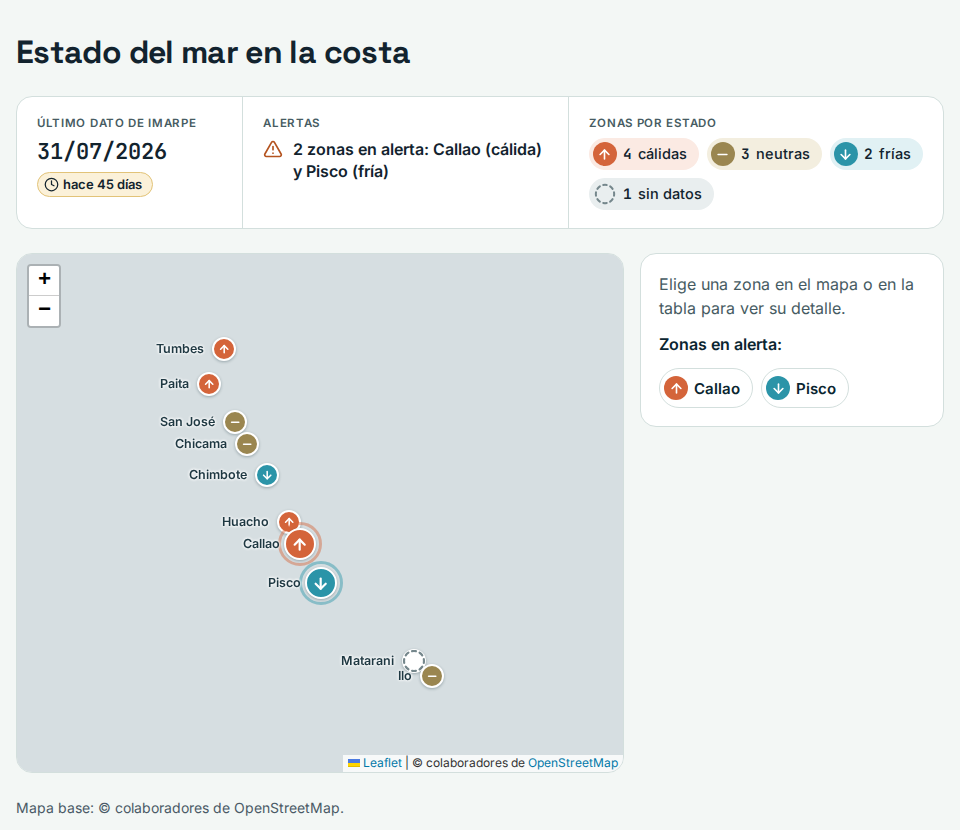
\includegraphics[width=0.82\textwidth]{figuras/inicio-top.png}\caption{Pantalla de inicio: resumen, mapa y zonas en alerta (RF-04).}\label{fig:inicio}\end{figure}

\begin{figure}[H]\centering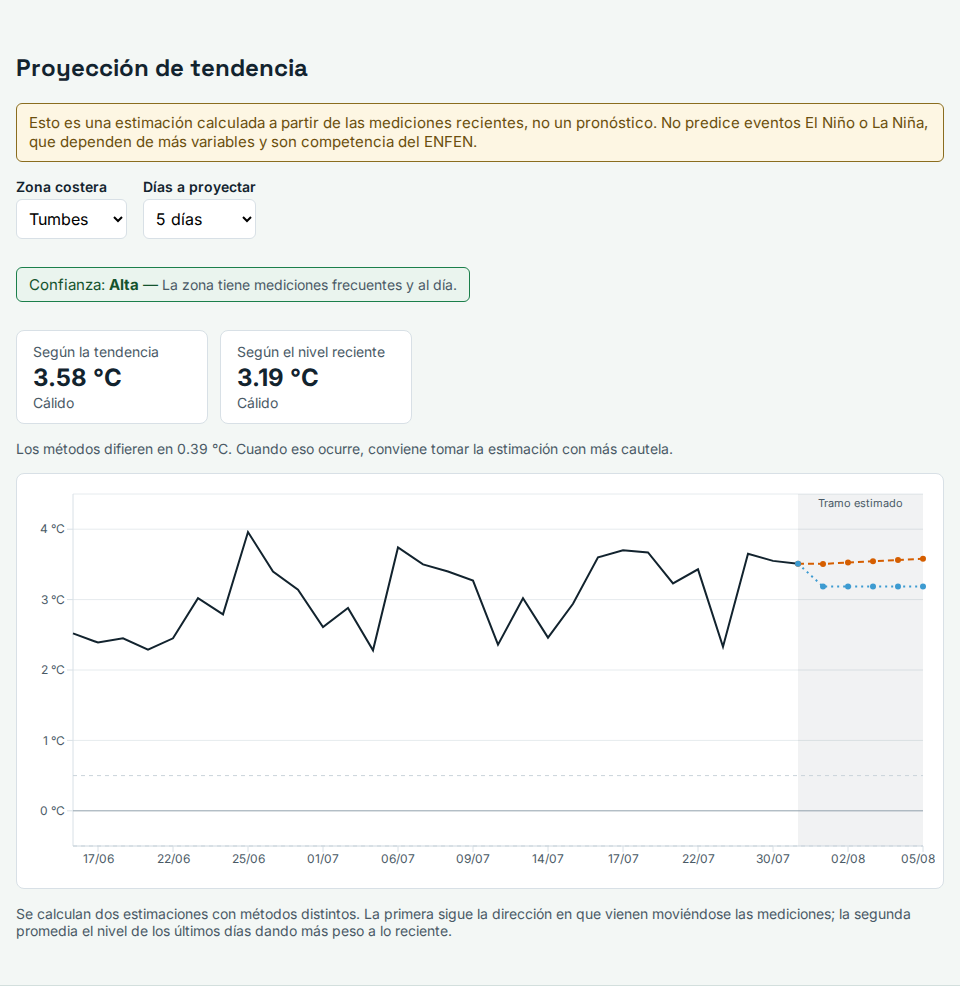
\includegraphics[width=0.72\textwidth]{figuras/proyeccion.png}\caption{Proyección de tendencia con dos estimaciones y tramo estimado sombreado (RF-02).}\label{fig:proy}\end{figure}

\begin{figure}[H]\centering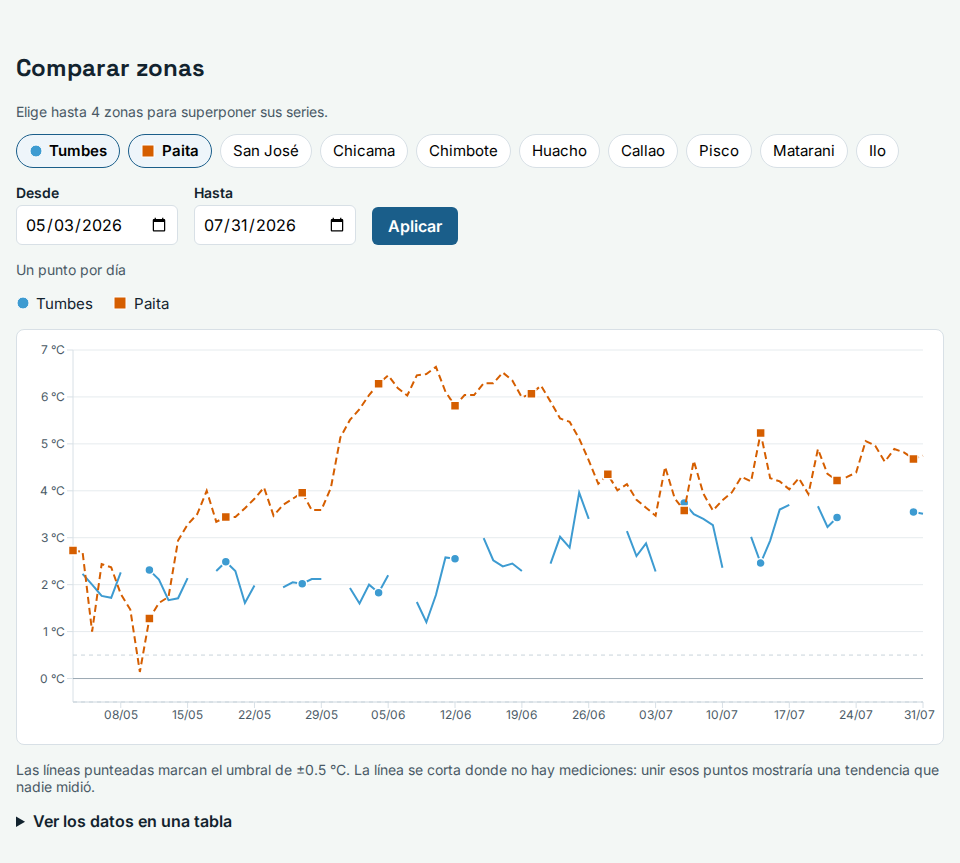
\includegraphics[width=0.72\textwidth]{figuras/comparacion.png}\caption{Comparación de laboratorios con series distinguidas por color, marcador y trazo (RF-06).}\label{fig:comp}\end{figure}

\clearpage\section{Historial de cambios de la línea base de requisitos}

Antes de esta versión, los requisitos funcionales se mantuvieron en la Especificación de Requisitos de Software del proyecto, cuya última línea base fue la v1.6. La Tabla \ref{tab:hist} registra los cambios de esa línea base, que este catálogo incorpora.



\Needspace{24\baselineskip}
{\footnotesize
\begin{xltabular}{\textwidth}{@{}>{\sffamily\bfseries}p{1.2cm}>{\raggedright\arraybackslash}p{1.7cm}>{\raggedright\arraybackslash}p{1.7cm}YY@{}}
\caption{Historial de cambios de la línea base de requisitos}\label{tab:hist}\\
\rowcolor{abisal}\textcolor{white}{\sffamily\bfseries\footnotesize Versión} & \textcolor{white}{\sffamily\bfseries\footnotesize Fecha} & \textcolor{white}{\sffamily\bfseries\footnotesize RF} & \textcolor{white}{\sffamily\bfseries\footnotesize Cambio} & \textcolor{white}{\sffamily\bfseries\footnotesize Motivo}\\
\endfirsthead
\rowcolor{abisal}\multicolumn{5}{@{}l@{}}{\textcolor{white}{\sffamily\footnotesize Historial de cambios de la línea base de requisitos (continuación)}}\\
\rowcolor{abisal}\textcolor{white}{\sffamily\bfseries\footnotesize Versión} & \textcolor{white}{\sffamily\bfseries\footnotesize Fecha} & \textcolor{white}{\sffamily\bfseries\footnotesize RF} & \textcolor{white}{\sffamily\bfseries\footnotesize Cambio} & \textcolor{white}{\sffamily\bfseries\footnotesize Motivo}\\
\endhead
1.0 & 10/09/2026 & — & Catálogo inicial de requisitos funcionales RF-01 a RF-08. & Línea base del proyecto.\\ \hline
\rowcolor{zebra}1.1 & 10/09/2026 & — & Se incorpora el control de versiones del catálogo. & Registrar con fecha y motivo cualquier cambio posterior.\\ \hline
1.2 & 10/09/2026 & RF-08 & Se elimina la importación programada; solo carga manual. Se define la importación parcial y la reimportación sin duplicados. & IMARPE publica sin frecuencia garantizada; un planificador no aportaba valor demostrable.\\ \hline
\rowcolor{zebra}1.3 & 10/09/2026 & RF-01, RF-04 & Racha por registros con tolerancia de 2 días; estado del mapa por promedio de 5 días; «sin datos recientes» a los 7 días. & El dataset tiene huecos y se publica con retraso; con el reloj del servidor todas las zonas quedarían sin clasificar.\\ \hline
1.4 & 10/09/2026 & RF-05, RF-06 & Agrupado automático de series; máximo de 4 zonas; identidad por color, forma y trazo. & Una serie de 56 años tiene hasta 16,678 puntos; más de 4 líneas no se leen; solo color excluye a personas con daltonismo.\\ \hline
\rowcolor{zebra}1.5 & 10/09/2026 & RF-02 & Se implementan ambos modelos; horizonte de 5 días; ventana y pesos definidos; indicador de confianza y tres señales visuales. & La discrepancia entre modelos mide la incertidumbre; una estimación con datos antiguos aparenta una validez que no tiene.\\ \hline
1.6 & 10/09/2026 & RF-03 & Se elimina el SMS; aviso de fin de episodio; registro separado del envío; reintento de fallidos. & El SMS tiene costo por mensaje; un correo caído no debe bloquear la evaluación.\\ \hline
\end{xltabular}}
\vspace{0.6em}

\end{document}